% !TEX program = xelatex
\documentclass[UTF8,fontset=fandol,a4paper,11pt]{ctexart}
\usepackage[margin=21mm,top=23mm,bottom=22mm,headheight=16pt]{geometry}
\usepackage{amsmath,amssymb,mathtools,bm}
\usepackage{tikz}
\usetikzlibrary{arrows.meta,calc,angles,quotes,patterns}
\usepackage{xcolor,booktabs,array,longtable,enumitem,fancyhdr,needspace}
\usepackage[unicode,hidelinks]{hyperref}
\definecolor{ink}{HTML}{24343C}
\definecolor{accent}{HTML}{166A70}
\definecolor{muted}{HTML}{65747A}
\definecolor{rulegray}{HTML}{D4DDE0}
\definecolor{warm}{HTML}{966037}
\color{ink}
\setlength{\parindent}{2em}
\setlength{\parskip}{4pt}
\linespread{1.12}
\AtBeginDocument{\setlength{\abovedisplayskip}{6pt plus 2pt minus 1pt}
\setlength{\belowdisplayskip}{6pt plus 2pt minus 1pt}
\setlength{\abovedisplayshortskip}{0pt plus 1pt}
\setlength{\belowdisplayshortskip}{4pt plus 1pt}}
\setlist[enumerate]{label=(\arabic*),leftmargin=2.3em,itemsep=3pt,topsep=4pt}
\setlist[itemize]{leftmargin=2em,itemsep=2pt,topsep=4pt}
\allowdisplaybreaks[1]
\setlength{\emergencystretch}{2em}
\setcounter{secnumdepth}{0}
\providecommand{\tightlist}{\setlength{\itemsep}{0pt}\setlength{\parskip}{0pt}}
\ctexset{section={format=\Large\bfseries\color{accent},beforeskip=10pt,afterskip=9pt},
subsection={format=\normalsize\bfseries\color{accent},beforeskip=10pt,afterskip=4pt},
subsubsection={format=\normalsize\bfseries,beforeskip=8pt,afterskip=3pt}}
\pagestyle{fancy}
\fancyhf{}
\fancyhead[L]{\small\color{muted}物理学难题集萃}
% 页眉仅保留书名；版本名称只在封面显示。
\fancyfoot[L]{\small\color{muted}\chapterlabel}
\fancyfoot[R]{\small\thepage}
\renewcommand{\headrulewidth}{0.4pt}
\renewcommand{\footrulewidth}{0pt}
\newcommand{\dd}{\mathop{}\!\mathrm{d}}
\newcommand{\vect}[1]{\bm{#1}}
\newcommand{\tagline}[1]{\noindent{\small\color{muted}#1}\par}
\newcommand{\result}[1]{\begin{equation*}\boxed{#1}\end{equation*}}
\newcommand{\figcaption}[1]{\par\vspace{2pt}{\small\color{muted}#1}\par}
\newcommand{\teach}[2]{\Needspace{4\baselineskip}\subsection*{讲解要点与追问}#1\par\smallskip\noindent\textbf{追问：}#2\par}
\newcommand{\workarea}{\par\vspace{7mm}\noindent{\small\color{muted}作答区}\par\vspace{4mm}
\noindent\textcolor{rulegray}{\rule{\linewidth}{0.3pt}}\par\vspace{16mm}
\noindent\textcolor{rulegray}{\rule{\linewidth}{0.3pt}}\par\vspace{16mm}
\noindent\textcolor{rulegray}{\rule{\linewidth}{0.3pt}}\par\vspace{16mm}
\noindent\textcolor{rulegray}{\rule{\linewidth}{0.3pt}}}
\tikzset{axis/.style={-{Stealth[length=2mm]},thin,color=muted},
motion/.style={-{Stealth[length=2.3mm]},thick,color=accent},
force/.style={-{Stealth[length=2.3mm]},thick,color=warm},
traj/.style={thick,color=accent},guide/.style={dashed,thin,color=muted},
object/.style={thick,color=ink},every node/.style={font=\small}}\widowpenalty=10000\clubpenalty=10000\displaywidowpenalty=10000\newcommand{\chapterlabel}{光学第一章\quad 几何光学}







\hypersetup{pdftitle={光学第一章 几何光学·学生版},pdfauthor={}}

\begin{document}\pdfbookmark[0]{光学第一章 几何光学}{cover}

\thispagestyle{empty}\vspace*{22mm}
\noindent{\Huge\bfseries 物理学难题集萃}\par\vspace{10mm}
\noindent{\LARGE 光学第一章}\par\vspace{6mm}
\noindent{\LARGE 几何光学}\par\vspace{12mm}
\noindent{\Large\color{accent}学生版}\par\vspace{9mm}
\noindent\textcolor{accent}{\rule{\linewidth}{1pt}}\par\vspace{9mm}
\noindent 第1--42题\par\vfill\clearpage
\pdfbookmark[1]{题目目录}{contents}\section*{题目目录}
\begin{longtable}{@{}r p{113mm} r@{}}\toprule 题号 & 题目 & 页码\\\midrule

\hyperref[q:1]{1} & \hyperref[q:1]{半圆柱玻璃的透光弧段} & \pageref{q:1} \\

\hyperref[q:2]{2} & \hyperref[q:2]{充液玻璃管的表观壁厚} & \pageref{q:2} \\

\hyperref[q:3]{3} & \hyperref[q:3]{水滴的一次内反射与最小偏向} & \pageref{q:3} \\

\hyperref[q:4]{4} & \hyperref[q:4]{温度计内径的表观尺寸} & \pageref{q:4} \\

\hyperref[q:5]{5} & \hyperref[q:5]{两平面镜的连续成像与可见范围} & \pageref{q:5} \\

\hyperref[q:6]{6} & \hyperref[q:6]{浸水截顶棱镜的全反射与像转动} & \pageref{q:6} \\

\hyperref[q:7]{7} & \hyperref[q:7]{跑道上方的梯度折射与可见距离} & \pageref{q:7} \\

\hyperref[q:8]{8} & \hyperref[q:8]{变折射率平板中的圆弧光路} & \pageref{q:8} \\

\hyperref[q:9]{9} & \hyperref[q:9]{热地面上方的下现蜃景} & \pageref{q:9} \\

\hyperref[q:10]{10} & \hyperref[q:10]{海面上方的上现蜃景} & \pageref{q:10} \\

\hyperref[q:11]{11} & \hyperref[q:11]{梯度光纤中的正弦光路} & \pageref{q:11} \\

\hyperref[q:12]{12} & \hyperref[q:12]{球面折射的光程驻值} & \pageref{q:12} \\

\hyperref[q:13]{13} & \hyperref[q:13]{无球差平凸透镜的曲面} & \pageref{q:13} \\

\hyperref[q:14]{14} & \hyperref[q:14]{绕地表圆弧传播所需的大气密度} & \pageref{q:14} \\

\hyperref[q:15]{15} & \hyperref[q:15]{弯月透镜的非近轴成像点} & \pageref{q:15} \\

\hyperref[q:16]{16} & \hyperref[q:16]{鱼缸直接像与反射像的速度} & \pageref{q:16} \\

\hyperref[q:17]{17} & \hyperref[q:17]{玻璃半球的两条反射成像光路} & \pageref{q:17} \\

\hyperref[q:18]{18} & \hyperref[q:18]{水杯与薄透镜的复合成像} & \pageref{q:18} \\

\hyperref[q:19]{19} & \hyperref[q:19]{透镜与平面镜的往返成像} & \pageref{q:19} \\

\hyperref[q:20]{20} & \hyperref[q:20]{用会聚光束测凹透镜焦距} & \pageref{q:20} \\

\hyperref[q:21]{21} & \hyperref[q:21]{直角棱镜与两透镜系统} & \pageref{q:21} \\

\hyperref[q:22]{22} & \hyperref[q:22]{自准直测定透镜折射率} & \pageref{q:22} \\

\hyperref[q:23]{23} & \hyperref[q:23]{注水表壳与球面镜的往返成像} & \pageref{q:23} \\

\hyperref[q:24]{24} & \hyperref[q:24]{双凸透镜后表面反射的自共轭} & \pageref{q:24} \\

\hyperref[q:25]{25} & \hyperref[q:25]{贴在水槽内外的平凸透镜} & \pageref{q:25} \\

\hyperref[q:26]{26} & \hyperref[q:26]{球面物的像何时仍为球面} & \pageref{q:26} \\

\hyperref[q:27]{27} & \hyperref[q:27]{厚透镜的主平面与两色有效焦距} & \pageref{q:27} \\

\hyperref[q:28]{28} & \hyperref[q:28]{玻璃球的焦点与表面物成像} & \pageref{q:28} \\

\hyperref[q:29]{29} & \hyperref[q:29]{正负透镜组的主点与重合虚像} & \pageref{q:29} \\

\hyperref[q:30]{30} & \hyperref[q:30]{远摄镜头的长焦与短镜筒} & \pageref{q:30} \\

\hyperref[q:31]{31} & \hyperref[q:31]{相机的景深与弥散圆} & \pageref{q:31} \\

\hyperref[q:32]{32} & \hyperref[q:32]{带场镜望远镜的出瞳与匹配} & \pageref{q:32} \\

\hyperref[q:33]{33} & \hyperref[q:33]{显微镜的放大率与调节焦深} & \pageref{q:33} \\

\hyperref[q:34]{34} & \hyperref[q:34]{惠更斯目镜的光阑与出瞳} & \pageref{q:34} \\

\hyperref[q:35]{35} & \hyperref[q:35]{显微镜出瞳与角放大率的反比} & \pageref{q:35} \\

\hyperref[q:36]{36} & \hyperref[q:36]{冕牌与火石玻璃的胶合消色差} & \pageref{q:36} \\

\hyperref[q:37]{37} & \hyperref[q:37]{分离双透镜的一阶色散条件} & \pageref{q:37} \\

\hyperref[q:38]{38} & \hyperref[q:38]{开普勒望远镜的分辨与视场} & \pageref{q:38} \\

\hyperref[q:39]{39} & \hyperref[q:39]{朗伯圆盘的轴上照度} & \pageref{q:39} \\

\hyperref[q:40]{40} & \hyperref[q:40]{物像亮度与折射率的关系} & \pageref{q:40} \\

\hyperref[q:41]{41} & \hyperref[q:41]{相机照度与相对孔径} & \pageref{q:41} \\

\hyperref[q:42]{42} & \hyperref[q:42]{透镜聚焦太阳光的照度} & \pageref{q:42} \\

\bottomrule\end{longtable}

\clearpage

\pdfbookmark[2]{第 1 题 半圆柱玻璃的透光弧段}{q1}

\section*{第 1 题\quad 半圆柱玻璃的透光弧段}\label{q:1}

折射率为$n=\sqrt2$的半圆柱玻璃置于空气中。在垂直于柱轴的截面内，一束平行光以$45^\circ$入射到平直表面上。求光线第一次到达圆弧表面时能够透出的弧段，以圆心角表示。图中$\phi$从右侧半径沿下半圆向左计量。

\begin{center}\begin{minipage}{.98\linewidth}\centering
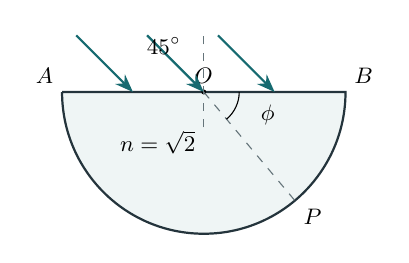
\begin{tikzpicture}[scale=.9,transform shape]
\fill[accent!7] (-2,0) arc(180:360:2)--cycle;\draw[object] (-2,0)--(2,0) arc(0:-180:2);\fill (0.00000,0.00000) circle(.035);\node[above] at (0.00000,0.00000) {$O$};\node[above left] at (-2.00000,0.00000) {$A$};\node[above right] at (2.00000,0.00000) {$B$};\draw[motion] (-1.80000,0.80000)--(-1.00000,0.00000);\draw[motion] (-0.80000,0.80000)--(0.00000,0.00000);\draw[motion] (0.20000,0.80000)--(1.00000,0.00000);\draw[guide] (0.00000,-0.50000)--(0.00000,0.90000);\node[left] at (-0.20000,0.65000) {$45^\circ$};\draw[guide] (0.00000,0.00000)--(1.28558,-1.53209);\node[below right] at (1.28558,-1.53209) {$P$};\draw[thin] (.5,0) arc(0:-50:.5);\node[right] at (0.67973,-0.31696) {$\phi$};\node[above] at (-0.65000,-1.00000) {$n=\sqrt2$};
\end{tikzpicture}
\figcaption{图光1.1\quad 平直面入射及下半圆的位置角}
\end{minipage}\end{center}

\workarea

\clearpage

\pdfbookmark[2]{第 2 题 充液玻璃管的表观壁厚}{q2}

\section*{第 2 题\quad 充液玻璃管的表观壁厚}\label{q:2}

内半径$r$、外半径$R$的圆柱玻璃管，玻璃折射率为$n_1>1$，管内充满折射率$n_2\ge1$的发光液体。观察者在空气中从侧面远处观察。求管壁的表观厚度恰好消失时$r$与$R$应满足的条件，并讨论$n_2<n_1$和$n_2\ge n_1$两种情形。

\begin{center}\begin{minipage}{.98\linewidth}\centering
\begin{tikzpicture}[scale=.9,transform shape]
\draw[object] (0.00000,0.00000) circle(2.00000);\draw[object] (0.00000,0.00000) circle(1.50000);\draw[<->,thin,color=muted] (0.00000,0.00000)--(2.00000,0.00000);\node[below] at (1.00000,0.00000) {$R$};\draw[<->,thin,color=muted] (0.00000,0.00000)--(-1.14907,0.96418);\node[above] at (-0.57453,0.48209) {$r$};\node[above] at (-0.15000,1.05000) {$n_2$};\node[above] at (1.65000,0.60000) {$n_1$};\node[above] at (2.70000,-0.20000) {空气};\node[below] at (0.00000,-2.50000) {远处观察};
\end{tikzpicture}
\figcaption{图光1.2\quad 同心玻璃管及发光液体}
\end{minipage}\end{center}

\workarea

\clearpage

\pdfbookmark[2]{第 3 题 水滴的一次内反射与最小偏向}{q3}

\section*{第 3 题\quad 水滴的一次内反射与最小偏向}\label{q:3}

一条光线从空气射入折射率$n>1$的球形水滴，经过一次内表面反射后再射出。入射角为$\theta$，折射角为$r$，光线传播方向沿图示同一转向累计的偏转量记为$\delta$，不将超过$\pi$的累计量折回为两射线间的较小夹角。判断内反射是否为全反射，并求$\delta$取得内部极小值时$\theta$满足的条件；说明该极小值存在的折射率范围。

\begin{center}\begin{minipage}{.98\linewidth}\centering
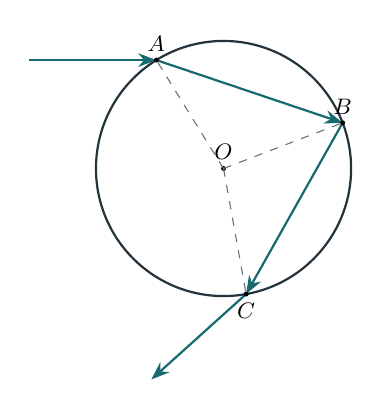
\begin{tikzpicture}[scale=.9,transform shape]
\draw[object] (0.00000,0.00000) circle(1.80000);\draw[motion] (-2.74821,1.53000)--(-0.94821,1.53000);
\draw[motion] (-0.94821,1.53000)--(1.68045,0.64505);
\draw[motion] (1.68045,0.64505)--(0.31909,-1.77149);
\draw[motion] (0.31909,-1.77149)--(-1.01859,-2.97591);\fill (0.00000,0.00000) circle(.035);\node[above] at (0.00000,0.00000) {$O$};\fill (-0.94821,1.53000) circle(.035);\node[above] at (-0.94821,1.53000) {$A$};\draw[guide] (0.00000,0.00000)--(-0.94821,1.53000);\fill (1.68045,0.64505) circle(.035);\node[above] at (1.68045,0.64505) {$B$};\draw[guide] (0.00000,0.00000)--(1.68045,0.64505);\fill (0.31909,-1.77149) circle(.035);\node[below] at (0.31909,-1.77149) {$C$};\draw[guide] (0.00000,0.00000)--(0.31909,-1.77149);
\end{tikzpicture}
\figcaption{图光1.3\quad 一折射、一次内反射、再折射的光支}
\end{minipage}\end{center}

\workarea

\clearpage

\pdfbookmark[2]{第 4 题 温度计内径的表观尺寸}{q4}

\section*{第 4 题\quad 温度计内径的表观尺寸}\label{q:4}

\begin{enumerate}
\item 一圆柱玻璃温度计的内、外直径分别为$2r=1\,\mathrm{mm}$、$2R=3\,\mathrm{mm}$，玻璃折射率$n_g=1.5$，外部为空气。从侧面远处观察，求内径的表观尺寸。
\item 另一温度计外径及玻璃折射率相同，内径为$2r=0.1\,\mathrm{mm}$，竖直悬在盛水圆柱烧杯的中心。水的折射率$n_w=4/3$，烧杯壁厚忽略。求从烧杯外侧远处观察时温度计内径和外径的表观尺寸。对细内径作近轴近似，并说明对外径采用的近似。

\item 在前两问中，另行区分两指定射线反延确定的径向虚像构造尺寸与垂直固定远处视线的投影尺寸；给出二者的联系和适用条件。
\end{enumerate}

\begin{center}\begin{minipage}{.98\linewidth}\centering
\begin{tikzpicture}[scale=.9,transform shape]
\draw[object] (0.00000,0.00000) circle(2.00000);\draw[object] (0.00000,0.00000) circle(0.66667);\fill (0.00000,0.00000) circle(.035);\node[below left] at (0.00000,0.00000) {$O$};\draw[<->,thin,color=muted] (-2.40000,-0.66667)--(-2.40000,0.66667);\node[left] at (-2.40000,0.00000) {$2r$};\draw[<->,thin,color=muted] (2.40000,-2.00000)--(2.40000,2.00000);\node[right] at (2.40000,0.00000) {$2R$};\node[above] at (0.00000,-1.30000) {$n_g$};\node[right] at (3.40000,0.00000) {观察};
\end{tikzpicture}
\figcaption{图光1.4\quad 圆柱温度计及内外径}
\end{minipage}\end{center}

\workarea

\clearpage

\pdfbookmark[2]{第 5 题 两平面镜的连续成像与可见范围}{q5}

\section*{第 5 题\quad 两平面镜的连续成像与可见范围}\label{q:5}

两块足够大的平面反射镜$A,B$相交，反射面相对，夹角为$0<\theta<\pi$。在垂直交棱的截面中，交点为$O$，物点$P$与$OA,OB$的夹角分别为$\alpha,\beta$，其中$\alpha+\beta=\theta$。观察者位于两镜之间。
\begin{enumerate}
\item 讨论一般情况下反射像的位置和最多可见像数的确定方法，区分不同方向形成的像与同一观察位置可见的像。
\item 当$\theta=\pi/5,\pi/3,\pi/2$时，各能形成多少个不同反射像，最多可见多少个？写出像的位置，并说明观察方向恰使光路经过交点$O$时的例外。
\end{enumerate}

\begin{center}\begin{minipage}{.98\linewidth}\centering
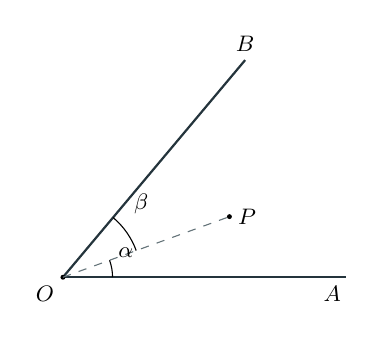
\begin{tikzpicture}[scale=.9,transform shape]
\draw[object] (0.00000,0.00000)--(4.00000,0.00000);\draw[object] (0.00000,0.00000)--(2.57115,3.06418);\fill (0.00000,0.00000) circle(.035);\node[below left] at (0.00000,0.00000) {$O$};\fill (2.34923,0.85505) circle(.035);\node[right] at (2.34923,0.85505) {$P$};\draw[guide] (0.00000,0.00000)--(2.34923,0.85505);\draw[thin] (.7,0) arc(0:20:.7);\draw[thin] (20:1.1) arc(20:50:1.1);\node[above] at (0.88633,0.15628) {$\alpha$};\node[above] at (1.10586,0.77433) {$\beta$};\node[below] at (3.80000,0.00000) {$A$};\node[above] at (2.57115,3.06418) {$B$};
\end{tikzpicture}
\figcaption{图光1.5\quad 镜间物点与两侧夹角}
\end{minipage}\end{center}

\workarea

\clearpage

\pdfbookmark[2]{第 6 题 浸水截顶棱镜的全反射与像转动}{q6}

\section*{第 6 题\quad 浸水截顶棱镜的全反射与像转动}\label{q:6}

折射率$n=1.50$的等腰玻璃三棱镜顶端截去，底面浸在折射率$n_w=1.33$的水中。两侧斜面与底面的夹角均为$\theta$，从左方入射的平行光与底面平行。
\begin{enumerate}
\item 求光线在底面发生全反射所需的最小$\theta$。
\item 通过该棱镜观察远物，若棱镜绕入射光轴以角速度$\omega$转动，描述所观察到的像转动。
\end{enumerate}

\begin{center}\begin{minipage}{.98\linewidth}\centering
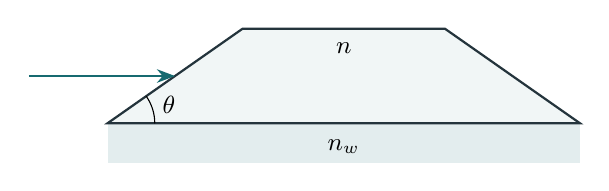
\begin{tikzpicture}[scale=1.0,font=\small]
\fill[accent!12](-3,-.5)rectangle(3,0);
\fill[accent!6](-3,0)--(3,0)--(1.28622239,1.20000000)--(-1.28622239,1.20000000)--cycle;
\draw[object](-3,0)--(3,0)--(1.28622239,1.20000000)--(-1.28622239,1.20000000)--cycle;
\draw[motion](-4,.6)--(-2.14311120,0.60000000);
\draw[thin](-2.4,0)arc(0:35:.6);
\node at(-2.22,.24){$\theta$};
\node at(0,.95){$n$};\node at(0,-.3){$n_w$};
\end{tikzpicture}
\figcaption{图光1.6\quad 截顶棱镜与浸水底面}
\end{minipage}\end{center}

\workarea

\clearpage

\pdfbookmark[2]{第 7 题 跑道上方的梯度折射与可见距离}{q7}

\section*{第 7 题\quad 跑道上方的梯度折射与可见距离}\label{q:7}

机场跑道上方空气的折射率随高度$y$变化为
\[
n(y)=n_0(1+ay),\qquad a=1.5\times10^{-6}\,\mathrm{m}^{-1}.
\]
一人站在跑道上，眼睛距地面$h=1.7\,\mathrm m$。忽略地球曲率，求他能看到的跑道最远距离$d$。给出光线轨迹和采用的近似。

\begin{center}\begin{minipage}{.98\linewidth}\centering
\begin{tikzpicture}[scale=.9,transform shape]
\draw[axis] (0.00000,0.00000)--(6.00000,0.00000);\draw[axis] (0.00000,0.00000)--(0.00000,2.50000);\node[above] at (0.00000,2.50000) {$y$};\node[below] at (6.00000,0.00000) {跑道};\fill (5.00000,2.00000) circle(.035);\node[right] at (5.00000,2.00000) {$E$};\draw[<->,thin,color=muted] (5.45000,0.00000)--(5.45000,2.00000);\node[right] at (5.45000,1.00000) {$h$};\draw[<->,thin,color=muted] (0.00000,-0.50000)--(5.00000,-0.50000);\node[below] at (2.50000,-0.50000) {$d$};
\end{tikzpicture}
\figcaption{图光1.7\quad 眼高与最远可见地面点；水平距离与高度分别缩放}
\end{minipage}\end{center}

\workarea

\clearpage

\pdfbookmark[2]{第 8 题 变折射率平板中的圆弧光路}{q8}

\section*{第 8 题\quad 变折射率平板中的圆弧光路}\label{q:8}

平板玻璃中折射率随水平坐标$x$变化：
\[
n(x)=\frac{n_0}{1-x/r},\qquad n_0=1.2,\quad r=13\,\mathrm{cm}.
\]
光线在$(0,0)$处沿$+y$轴进入玻璃，从上表面的$A$点进入空气，与上表面外法线成$\alpha=30^\circ$。求玻璃内光线轨迹、$A$点折射率和板厚$d$，取$0\le x<r$的光路。

\begin{center}\begin{minipage}{.98\linewidth}\centering
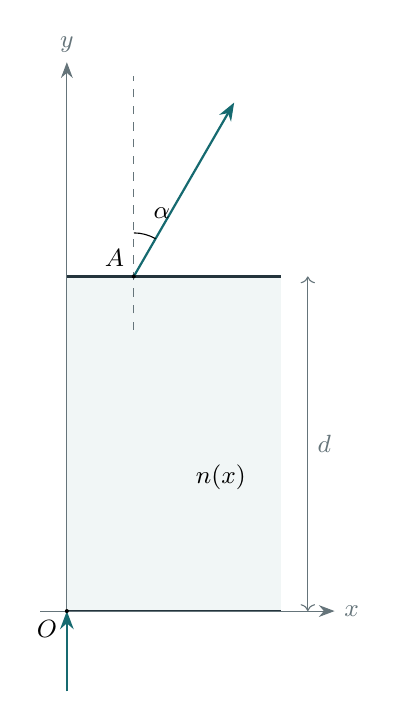
\begin{tikzpicture}[scale=.85,font=\small]
\fill[accent!6](0,0)rectangle(3.2,5);
\draw[object](0,0)--(3.2,0);\draw[object](0,5)--(3.2,5);
\draw[axis](-.4,0)--(4,0)node[right]{$x$};
\draw[axis](0,-.6)--(0,8.2)node[above]{$y$};
\draw[motion](0,-1.2)--(0,0);
\draw[guide](1,4.2)--(1,8.0);
\draw[motion](1,5)--(2.5,7.598076211);
\draw($(1,5)+(60:.65)$)arc(60:90:.65);
\node at(1.42,5.95){$\alpha$};
\fill(0,0)circle(.03);\node[below left]at(0,0){$O$};
\fill(1,5)circle(.03);\node[above left]at(1,5){$A$};
\node at(2.3,2){$n(x)$};
\draw[<->,color=muted](3.6,0)--(3.6,5)node[midway,right]{$d$};
\end{tikzpicture}
\figcaption{图光1.8\quad 随横坐标变化的介质与上表面出口}
\end{minipage}\end{center}

\workarea

\clearpage

\pdfbookmark[2]{第 9 题 热地面上方的下现蜃景}{q9}

\section*{第 9 题\quad 热地面上方的下现蜃景}\label{q:9}

白天沙漠近地空气较热，折射率随高度增加而增大，取模型
\[
n^2(y)=n_0^2+n_p^2(1-e^{-\alpha y}),\qquad y\ge0,\quad \alpha>0,\ n_p>0.
\]
物点$P$位于$(0,H)$。考虑从$P$向右下方发出、与竖直方向成$\theta_1$角的光线，$0<\theta_1<\pi/2$。求其轨迹，讨论能否在地面上方转向，并结合光线图解释下现蜃景。

\begin{center}\begin{minipage}{.98\linewidth}\centering
\begin{tikzpicture}[scale=.9,font=\small]
\draw[axis](0,0)--(6.8,0)node[right]{$x$};
\draw[axis](0,0)--(0,3.4)node[above]{$y$};
\foreach \a in{.5,1,1.5,2,2.5}{\draw[guide](.3,\a)--(2.6,\a);}
\fill(0,2.7)circle(.035);\node[left]at(0,2.7){$P=(0,H)$};
\draw[motion](0,2.7)--(2,1.545299462);
\draw($(0,2.7)+(-90:.75)$)arc(-90:-30:.75);
\node at(.51,1.8){$\theta_1$};
\draw[<->,color=muted](-.6,0)--(-.6,2.7)node[midway,left]{$H$};
\node[align=left,anchor=west]at(3.0,2.8){层间法线竖直\\$\theta_1$从向下竖直方向量取\\能否转向还须计算守恒量};
\end{tikzpicture}
\figcaption{图光1.9\quad 水平分层与从高处向下发出的光}
\end{minipage}\end{center}

\workarea

\clearpage

\pdfbookmark[2]{第 10 题 海面上方的上现蜃景}{q10}

\section*{第 10 题\quad 海面上方的上现蜃景}\label{q:10}

湿冷海面上方的空气折射率随高度减小，取
\[
n^2(y)=n_0^2+n_p^2e^{-\alpha y},\qquad y\ge0,\quad n_p,\alpha>0.
\]
物点位于$(0,y_0)$。求从物点向右上方发出的光线轨迹，初始与竖直方向夹角为$\theta_1$，$0<\theta_1<\pi/2$；讨论能否在空中转向，并解释上现蜃景。

\begin{center}\begin{minipage}{.98\linewidth}\centering
\begin{tikzpicture}[scale=.9,font=\small]
\draw[axis](0,0)--(6.6,0)node[right]{$x$};
\draw[axis](0,0)--(0,3.4)node[above]{$y$};
\foreach \q in{.5,1,1.5,2,2.5,3}{\draw[guide](.25,\q)--(2.55,\q);}
\fill(0,1.2)circle(.035);\node[above left]at(0,1.2){$P=(0,y_0)$};
\draw[motion](0,1.2)--(1.6,2.123760431);
\draw($(0,1.2)+(30:.65)$)arc(30:90:.65);
\node[fill=white,inner sep=1pt]at(.42,2.02){$\theta_1$};
\draw[<->,color=muted](-.65,0)--(-.65,1.2)node[midway,left]{$y_0$};
\node[anchor=west,align=left]at(3.15,2.2){层间法线沿竖直方向\\$\theta_1$从向上法线量起\\先判$n_1\sin\theta_1$与$n_0$的大小};
\end{tikzpicture}
\figcaption{图光1.10\quad 冷海面上方的上升发射光}
\end{minipage}\end{center}

\workarea

\clearpage

\pdfbookmark[2]{第 11 题 梯度光纤中的正弦光路}{q11}

\section*{第 11 题\quad 梯度光纤中的正弦光路}\label{q:11}

光纤折射率沿径向分布为
\[
n^2(r)=n_0^2(1-a^2r^2),
\]
其中$a$具有长度倒数的量纲，工作区域满足$ar<1$。求从轴上$O$点进入、位于含轴截面的光线轨迹；初始光线与轴线的夹角为$\eta_0$，$|\eta_0|<\pi/2$。说明小角度自聚焦，并讨论不通过轴线的光线能否一概视为平面曲线。

\begin{center}\begin{minipage}{.98\linewidth}\centering
\begin{tikzpicture}[scale=.9,font=\small]
\draw[object](0,-1.3)--(7,-1.3);\draw[object](0,1.3)--(7,1.3);
\draw[axis](-.3,0)--(7.5,0)node[right]{$x$};
\draw[axis](0,-1.6)--(0,1.85)node[above]{$z$};
\fill(0,0)circle(.035);\node[below left]at(0,0){$O$};
\draw[motion](0,0)--(1.879385242,.684040287);
\draw(1,0)arc(0:20:1);\node[fill=white,inner sep=1pt]at(.88,.38){$\eta_0$};
\node[align=left,anchor=west,fill=white]at(3.0,.7){$\eta_0$从正$x$轴量起\\横向坐标$z$有正负，$r=|z|$\\纤芯内$n^2=n_0^2(1-a^2z^2)$};
\end{tikzpicture}
\figcaption{图光1.11\quad 子午截面的入射点与带符号横向位移}
\end{minipage}\end{center}

\workarea

\clearpage

\pdfbookmark[2]{第 12 题 球面折射的光程驻值}{q12}

\section*{第 12 题\quad 球面折射的光程驻值}\label{q:12}

一球面分隔折射率为$n_1<n_2$的两介质，球面顶点为$O$，曲率中心$C$位于右侧，$OC=R>0$。轴上物点$Q$在$O$左方，$OQ=s$；考察右侧轴上点$Q'$，$OQ'=s'$。在近轴条件下，求哪些从$Q$发出的光线能经球面折射到$Q'$，光程取何种驻值，并求$Q'$成为像点的条件。

\begin{center}\begin{minipage}{.98\linewidth}\centering
\begin{tikzpicture}[x=.65cm,y=2.8cm,font=\small]
\draw[axis](-3.5,0)--(7.2,0);
\draw[object]plot coordinates {(0.122417438,-0.479425539) (0.117667141,-0.470625888) (0.113005077,-0.461779176) (0.108431712,-0.452886285) (0.103947502,-0.443948107) (0.099552898,-0.434965534) (0.095248337,-0.425939465) (0.091034250,-0.416870802) (0.086911060,-0.407760453) (0.082879177,-0.398609328) (0.078939006,-0.389418342) (0.075090940,-0.380188415) (0.071335364,-0.370920469) (0.067672654,-0.361615432) (0.064103176,-0.352274233) (0.060627287,-0.342897807) (0.057245334,-0.333487092) (0.053957656,-0.324043028) (0.050764582,-0.314566561) (0.047666430,-0.305058636) (0.044663511,-0.295520207) (0.041756124,-0.285952225) (0.038944562,-0.276355649) (0.036229104,-0.266731437) (0.033610022,-0.257080552) (0.031087578,-0.247403959) (0.028662025,-0.237702626) (0.026333605,-0.227977524) (0.024102551,-0.218229623) (0.021969085,-0.208459900) (0.019933422,-0.198669331) (0.017995765,-0.188858895) (0.016156307,-0.179029573) (0.014415233,-0.169182349) (0.012772717,-0.159318207) (0.011228922,-0.149438132) (0.009784004,-0.139543115) (0.008438106,-0.129634143) (0.007191364,-0.119712207) (0.006043902,-0.109778301) (0.004995835,-0.099833417) (0.004047267,-0.089878549) (0.003198294,-0.079914694) (0.002449000,-0.069942847) (0.001799460,-0.059964006) (0.001249740,-0.049979169) (0.000799893,-0.039989334) (0.000449966,-0.029995500) (0.000199993,-0.019998667) (0.000050000,-0.009999833) (0.000000000,0.000000000) (0.000050000,0.009999833) (0.000199993,0.019998667) (0.000449966,0.029995500) (0.000799893,0.039989334) (0.001249740,0.049979169) (0.001799460,0.059964006) (0.002449000,0.069942847) (0.003198294,0.079914694) (0.004047267,0.089878549) (0.004995835,0.099833417) (0.006043902,0.109778301) (0.007191364,0.119712207) (0.008438106,0.129634143) (0.009784004,0.139543115) (0.011228922,0.149438132) (0.012772717,0.159318207) (0.014415233,0.169182349) (0.016156307,0.179029573) (0.017995765,0.188858895) (0.019933422,0.198669331) (0.021969085,0.208459900) (0.024102551,0.218229623) (0.026333605,0.227977524) (0.028662025,0.237702626) (0.031087578,0.247403959) (0.033610022,0.257080552) (0.036229104,0.266731437) (0.038944562,0.276355649) (0.041756124,0.285952225) (0.044663511,0.295520207) (0.047666430,0.305058636) (0.050764582,0.314566561) (0.053957656,0.324043028) (0.057245334,0.333487092) (0.060627287,0.342897807) (0.064103176,0.352274233) (0.067672654,0.361615432) (0.071335364,0.370920469) (0.075090940,0.380188415) (0.078939006,0.389418342) (0.082879177,0.398609328) (0.086911060,0.407760453) (0.091034250,0.416870802) (0.095248337,0.425939465) (0.099552898,0.434965534) (0.103947502,0.443948107) (0.108431712,0.452886285) (0.113005077,0.461779176) (0.117667141,0.470625888) (0.122417438,0.479425539)};
\fill(-3,0)circle(1.1pt);\node[below]at(-3,0){$Q$};
\fill(0,0)circle(1.1pt);\node[below left]at(0,0){$O$};
\fill(1,0)circle(1.1pt);\node[below]at(1,0){$C$};
\fill(6,0)circle(1.1pt);\node[below]at(6,0){$Q'$};
\draw[motion,color=warm](-3,0)--(0.031087578,0.247403959);
\draw[motion,color=warm](0.031087578,0.247403959)--(6,0);
\fill(0.031087578,0.247403959)circle(1.1pt);\node[above left]at(0.031087578,0.247403959){$M$};
\draw[guide](1,0)--(-.453369633,.371105939);
\draw($(1,0)+(165.676055:.45)$)arc(165.676055:180:.45);
\node[fill=white,inner sep=1pt]at(.5,.09){$\vartheta$};
\draw[<->,color=muted](-3,-.45)--(0,-.45)node[midway,below]{$s$};
\draw[<->,color=muted](0,-.67)--(6,-.67)node[midway,below]{$s'$};
\node[anchor=west,align=left]at(8.1,.05){$OC=R,\ CM=R$\\$M=(R(1-\cos\vartheta),R\sin\vartheta)$\\$\vartheta$从$CO$的左向半径量起\\折线为候选路径，须另检驻值条件\\示意取$s'>R$，$s'-R$按实际位置取值\\横、纵分别缩放，不能据图量角};
\end{tikzpicture}
\figcaption{图光1.12\quad 候选折射点与两端轴上点}
\end{minipage}\end{center}

\workarea

\clearpage

\pdfbookmark[2]{第 13 题 无球差平凸透镜的曲面}{q13}

\section*{第 13 题\quad 无球差平凸透镜的曲面}\label{q:13}

折射率$n>1$的平凸透镜置于空气中，平面为$x=0$，光沿$+x$方向垂直入射。透镜孔径半径为$R$，曲面边缘在$(0,\pm R)$，要求全部入射平行光会聚于空气中的$F=(f,0)$。求曲面形状、轴上厚度$OA$，以及孔径$R$的限制；讨论极限情形。

\begin{center}\begin{minipage}{.98\linewidth}\centering
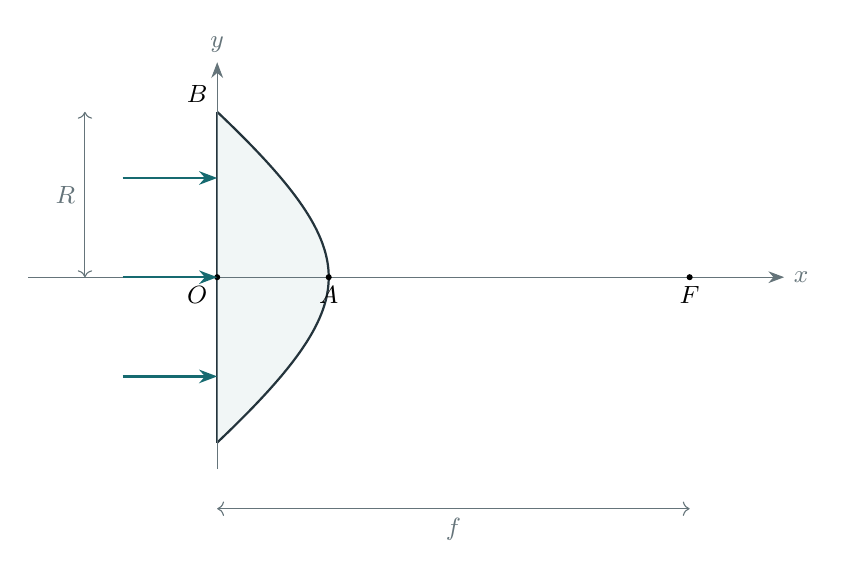
\begin{tikzpicture}[x=6cm,y=4.2cm,font=\small]
\fill[accent!6](0,-.5)--plot coordinates {(0.000000000,-0.500000000) (0.004095450,-0.494444444) (0.008176057,-0.488888889) (0.012241475,-0.483333333) (0.016291355,-0.477777778) (0.020325332,-0.472222222) (0.024343035,-0.466666667) (0.028344082,-0.461111111) (0.032328080,-0.455555556) (0.036294626,-0.450000000) (0.040243306,-0.444444444) (0.044173695,-0.438888889) (0.048085355,-0.433333333) (0.051977838,-0.427777778) (0.055850682,-0.422222222) (0.059703415,-0.416666667) (0.063535549,-0.411111111) (0.067346586,-0.405555556) (0.071136013,-0.400000000) (0.074903304,-0.394444444) (0.078647918,-0.388888889) (0.082369301,-0.383333333) (0.086066883,-0.377777778) (0.089740081,-0.372222222) (0.093388294,-0.366666667) (0.097010908,-0.361111111) (0.100607291,-0.355555556) (0.104176798,-0.350000000) (0.107718764,-0.344444444) (0.111232510,-0.338888889) (0.114717338,-0.333333333) (0.118172536,-0.327777778) (0.121597372,-0.322222222) (0.124991097,-0.316666667) (0.128352944,-0.311111111) (0.131682131,-0.305555556) (0.134977853,-0.300000000) (0.138239291,-0.294444444) (0.141465608,-0.288888889) (0.144655946,-0.283333333) (0.147809431,-0.277777778) (0.150925171,-0.272222222) (0.154002256,-0.266666667) (0.157039758,-0.261111111) (0.160036731,-0.255555556) (0.162992214,-0.250000000) (0.165905227,-0.244444444) (0.168774775,-0.238888889) (0.171599847,-0.233333333) (0.174379416,-0.227777778) (0.177112441,-0.222222222) (0.179797869,-0.216666667) (0.182434630,-0.211111111) (0.185021647,-0.205555556) (0.187557828,-0.200000000) (0.190042073,-0.194444444) (0.192473274,-0.188888889) (0.194850316,-0.183333333) (0.197172076,-0.177777778) (0.199437431,-0.172222222) (0.201645251,-0.166666667) (0.203794411,-0.161111111) (0.205883782,-0.155555556) (0.207912242,-0.150000000) (0.209878673,-0.144444444) (0.211781968,-0.138888889) (0.213621025,-0.133333333) (0.215394760,-0.127777778) (0.217102100,-0.122222222) (0.218741994,-0.116666667) (0.220313407,-0.111111111) (0.221815331,-0.105555556) (0.223246783,-0.100000000) (0.224606807,-0.094444444) (0.225894481,-0.088888889) (0.227108917,-0.083333333) (0.228249262,-0.077777778) (0.229314705,-0.072222222) (0.230304478,-0.066666667) (0.231217856,-0.061111111) (0.232054163,-0.055555556) (0.232812774,-0.050000000) (0.233493113,-0.044444444) (0.234094663,-0.038888889) (0.234616959,-0.033333333) (0.235059597,-0.027777778) (0.235422232,-0.022222222) (0.235704578,-0.016666667) (0.235906413,-0.011111111) (0.236027578,-0.005555556) (0.236067977,0.000000000) (0.236027578,0.005555556) (0.235906413,0.011111111) (0.235704578,0.016666667) (0.235422232,0.022222222) (0.235059597,0.027777778) (0.234616959,0.033333333) (0.234094663,0.038888889) (0.233493113,0.044444444) (0.232812774,0.050000000) (0.232054163,0.055555556) (0.231217856,0.061111111) (0.230304478,0.066666667) (0.229314705,0.072222222) (0.228249262,0.077777778) (0.227108917,0.083333333) (0.225894481,0.088888889) (0.224606807,0.094444444) (0.223246783,0.100000000) (0.221815331,0.105555556) (0.220313407,0.111111111) (0.218741994,0.116666667) (0.217102100,0.122222222) (0.215394760,0.127777778) (0.213621025,0.133333333) (0.211781968,0.138888889) (0.209878673,0.144444444) (0.207912242,0.150000000) (0.205883782,0.155555556) (0.203794411,0.161111111) (0.201645251,0.166666667) (0.199437431,0.172222222) (0.197172076,0.177777778) (0.194850316,0.183333333) (0.192473274,0.188888889) (0.190042073,0.194444444) (0.187557828,0.200000000) (0.185021647,0.205555556) (0.182434630,0.211111111) (0.179797869,0.216666667) (0.177112441,0.222222222) (0.174379416,0.227777778) (0.171599847,0.233333333) (0.168774775,0.238888889) (0.165905227,0.244444444) (0.162992214,0.250000000) (0.160036731,0.255555556) (0.157039758,0.261111111) (0.154002256,0.266666667) (0.150925171,0.272222222) (0.147809431,0.277777778) (0.144655946,0.283333333) (0.141465608,0.288888889) (0.138239291,0.294444444) (0.134977853,0.300000000) (0.131682131,0.305555556) (0.128352944,0.311111111) (0.124991097,0.316666667) (0.121597372,0.322222222) (0.118172536,0.327777778) (0.114717338,0.333333333) (0.111232510,0.338888889) (0.107718764,0.344444444) (0.104176798,0.350000000) (0.100607291,0.355555556) (0.097010908,0.361111111) (0.093388294,0.366666667) (0.089740081,0.372222222) (0.086066883,0.377777778) (0.082369301,0.383333333) (0.078647918,0.388888889) (0.074903304,0.394444444) (0.071136013,0.400000000) (0.067346586,0.405555556) (0.063535549,0.411111111) (0.059703415,0.416666667) (0.055850682,0.422222222) (0.051977838,0.427777778) (0.048085355,0.433333333) (0.044173695,0.438888889) (0.040243306,0.444444444) (0.036294626,0.450000000) (0.032328080,0.455555556) (0.028344082,0.461111111) (0.024343035,0.466666667) (0.020325332,0.472222222) (0.016291355,0.477777778) (0.012241475,0.483333333) (0.008176057,0.488888889) (0.004095450,0.494444444) (0.000000000,0.500000000)}--cycle;
\draw[object](0,-.5)--(0,.5);\draw[object]plot coordinates {(0.000000000,-0.500000000) (0.004095450,-0.494444444) (0.008176057,-0.488888889) (0.012241475,-0.483333333) (0.016291355,-0.477777778) (0.020325332,-0.472222222) (0.024343035,-0.466666667) (0.028344082,-0.461111111) (0.032328080,-0.455555556) (0.036294626,-0.450000000) (0.040243306,-0.444444444) (0.044173695,-0.438888889) (0.048085355,-0.433333333) (0.051977838,-0.427777778) (0.055850682,-0.422222222) (0.059703415,-0.416666667) (0.063535549,-0.411111111) (0.067346586,-0.405555556) (0.071136013,-0.400000000) (0.074903304,-0.394444444) (0.078647918,-0.388888889) (0.082369301,-0.383333333) (0.086066883,-0.377777778) (0.089740081,-0.372222222) (0.093388294,-0.366666667) (0.097010908,-0.361111111) (0.100607291,-0.355555556) (0.104176798,-0.350000000) (0.107718764,-0.344444444) (0.111232510,-0.338888889) (0.114717338,-0.333333333) (0.118172536,-0.327777778) (0.121597372,-0.322222222) (0.124991097,-0.316666667) (0.128352944,-0.311111111) (0.131682131,-0.305555556) (0.134977853,-0.300000000) (0.138239291,-0.294444444) (0.141465608,-0.288888889) (0.144655946,-0.283333333) (0.147809431,-0.277777778) (0.150925171,-0.272222222) (0.154002256,-0.266666667) (0.157039758,-0.261111111) (0.160036731,-0.255555556) (0.162992214,-0.250000000) (0.165905227,-0.244444444) (0.168774775,-0.238888889) (0.171599847,-0.233333333) (0.174379416,-0.227777778) (0.177112441,-0.222222222) (0.179797869,-0.216666667) (0.182434630,-0.211111111) (0.185021647,-0.205555556) (0.187557828,-0.200000000) (0.190042073,-0.194444444) (0.192473274,-0.188888889) (0.194850316,-0.183333333) (0.197172076,-0.177777778) (0.199437431,-0.172222222) (0.201645251,-0.166666667) (0.203794411,-0.161111111) (0.205883782,-0.155555556) (0.207912242,-0.150000000) (0.209878673,-0.144444444) (0.211781968,-0.138888889) (0.213621025,-0.133333333) (0.215394760,-0.127777778) (0.217102100,-0.122222222) (0.218741994,-0.116666667) (0.220313407,-0.111111111) (0.221815331,-0.105555556) (0.223246783,-0.100000000) (0.224606807,-0.094444444) (0.225894481,-0.088888889) (0.227108917,-0.083333333) (0.228249262,-0.077777778) (0.229314705,-0.072222222) (0.230304478,-0.066666667) (0.231217856,-0.061111111) (0.232054163,-0.055555556) (0.232812774,-0.050000000) (0.233493113,-0.044444444) (0.234094663,-0.038888889) (0.234616959,-0.033333333) (0.235059597,-0.027777778) (0.235422232,-0.022222222) (0.235704578,-0.016666667) (0.235906413,-0.011111111) (0.236027578,-0.005555556) (0.236067977,0.000000000) (0.236027578,0.005555556) (0.235906413,0.011111111) (0.235704578,0.016666667) (0.235422232,0.022222222) (0.235059597,0.027777778) (0.234616959,0.033333333) (0.234094663,0.038888889) (0.233493113,0.044444444) (0.232812774,0.050000000) (0.232054163,0.055555556) (0.231217856,0.061111111) (0.230304478,0.066666667) (0.229314705,0.072222222) (0.228249262,0.077777778) (0.227108917,0.083333333) (0.225894481,0.088888889) (0.224606807,0.094444444) (0.223246783,0.100000000) (0.221815331,0.105555556) (0.220313407,0.111111111) (0.218741994,0.116666667) (0.217102100,0.122222222) (0.215394760,0.127777778) (0.213621025,0.133333333) (0.211781968,0.138888889) (0.209878673,0.144444444) (0.207912242,0.150000000) (0.205883782,0.155555556) (0.203794411,0.161111111) (0.201645251,0.166666667) (0.199437431,0.172222222) (0.197172076,0.177777778) (0.194850316,0.183333333) (0.192473274,0.188888889) (0.190042073,0.194444444) (0.187557828,0.200000000) (0.185021647,0.205555556) (0.182434630,0.211111111) (0.179797869,0.216666667) (0.177112441,0.222222222) (0.174379416,0.227777778) (0.171599847,0.233333333) (0.168774775,0.238888889) (0.165905227,0.244444444) (0.162992214,0.250000000) (0.160036731,0.255555556) (0.157039758,0.261111111) (0.154002256,0.266666667) (0.150925171,0.272222222) (0.147809431,0.277777778) (0.144655946,0.283333333) (0.141465608,0.288888889) (0.138239291,0.294444444) (0.134977853,0.300000000) (0.131682131,0.305555556) (0.128352944,0.311111111) (0.124991097,0.316666667) (0.121597372,0.322222222) (0.118172536,0.327777778) (0.114717338,0.333333333) (0.111232510,0.338888889) (0.107718764,0.344444444) (0.104176798,0.350000000) (0.100607291,0.355555556) (0.097010908,0.361111111) (0.093388294,0.366666667) (0.089740081,0.372222222) (0.086066883,0.377777778) (0.082369301,0.383333333) (0.078647918,0.388888889) (0.074903304,0.394444444) (0.071136013,0.400000000) (0.067346586,0.405555556) (0.063535549,0.411111111) (0.059703415,0.416666667) (0.055850682,0.422222222) (0.051977838,0.427777778) (0.048085355,0.433333333) (0.044173695,0.438888889) (0.040243306,0.444444444) (0.036294626,0.450000000) (0.032328080,0.455555556) (0.028344082,0.461111111) (0.024343035,0.466666667) (0.020325332,0.472222222) (0.016291355,0.477777778) (0.012241475,0.483333333) (0.008176057,0.488888889) (0.004095450,0.494444444) (0.000000000,0.500000000)};
\draw[axis](-.4,0)--(1.2,0)node[right]{$x$};
\draw[axis](0,-.58)--(0,.65)node[above]{$y$};
\fill(0,0)circle(1.1pt);\node[below left]at(0,0){$O$};
\fill(0.236067977,0)circle(1.1pt);\node[below]at(0.236067977,0){$A$};
\fill(1,0)circle(1.1pt);\node[below]at(1,0){$F$};
\node[above left]at(0,.5){$B$};
\draw[<->,color=muted](-.28,0)--(-.28,.5)node[midway,left]{$R$};
\draw[<->,color=muted](0,-.7)--(1,-.7)node[midway,below]{$f$};
\foreach \Y in{-.3,0,.3}{\draw[motion](-.2,\Y)--(0,\Y);}
\end{tikzpicture}
\figcaption{图光1.13\quad 平面入口、孔径与外部焦点}
\end{minipage}\end{center}

\workarea

\clearpage

\pdfbookmark[2]{第 14 题 绕地表圆弧传播所需的大气密度}{q14}

\section*{第 14 题\quad 绕地表圆弧传播所需的大气密度}\label{q:14}

假设大气满足$n-1\propto\rho$，等温大气密度服从玻尔兹曼分布。若要使水平光线沿地球表面的圆弧弯曲传播，地表空气密度需为实际密度的多少倍？给定$T=300\,\mathrm K$，实际地表折射率$n_{\rm act}=1.0003$，空气平均摩尔质量$\mu=29\times10^{-3}\,\mathrm{kg\,mol^{-1}}$，地球半径$r_0=6.4\times10^6\,\mathrm m$，取$g=9.8\,\mathrm{m\,s^{-2}}$、气体常量$\mathcal R=8.31\,\mathrm{J\,mol^{-1}K^{-1}}$。

\begin{center}\begin{minipage}{.97\linewidth}\centering
\begin{tikzpicture}[scale=1]
\fill[accent!4](0,0)circle(1.7);\draw[object](0,0)circle(1.7);
\fill(0,0)circle(1.2pt);\node[below]at(0,0){$O$};
\draw[motion](35:1.7)arc(35:135:1.7);
\fill(35:1.7)circle(1.2pt);\node[above right]at(35:1.7){$A$};
\fill(135:1.7)circle(1.2pt);\node[above left]at(135:1.7){$B$};
\draw[guide](0,0)--(35:1.7)node[midway,below right]{$r_0$};
\draw(35:.5)arc(35:135:.5);\node[above]at(85:.5){$\Delta\varphi$};
\node[anchor=west,align=left]at(2.3,.3){目标光路：$r=r_0$\\光线处处沿圆周切线\\$n$随半径$r$增大而减小};
\end{tikzpicture}
\figcaption{图光1.14　地表目标圆弧及径向折射率分布}
\end{minipage}\end{center}


\workarea

\clearpage

\pdfbookmark[2]{第 15 题 弯月透镜的非近轴成像点}{q15}

\section*{第 15 题\quad 弯月透镜的非近轴成像点}\label{q:15}

弯月形透镜折射率为$n>1$，置于空气中。两球面$\Sigma_1,\Sigma_2$的曲率中心分别为$C_1,C_2$，后球面$\Sigma_2$的半径为$R$，$C_1$位于$C_2$左侧，且$C_1C_2=R/n$。物点$Q$恰在$C_1$。证明：从$Q$出发、能穿过所示有效球面区域的光线，包括非近轴光线，出射后的反向延长线均通过同一虚像点$Q'$；求$C_2Q'$。

\begin{center}\begin{minipage}{.97\linewidth}\centering
\begin{tikzpicture}[x=2.2cm,y=2.2cm,font=\small]
\fill[accent!6]plot coordinates {(0.429918943,-0.600000000) (0.433540385,-0.593333333) (0.437109679,-0.586666667) (0.440627332,-0.580000000) (0.444093834,-0.573333333) (0.447509661,-0.566666667) (0.450875279,-0.560000000) (0.454191140,-0.553333333) (0.457457684,-0.546666667) (0.460675340,-0.540000000) (0.463844525,-0.533333333) (0.466965647,-0.526666667) (0.470039100,-0.520000000) (0.473065271,-0.513333333) (0.476044534,-0.506666667) (0.478977257,-0.500000000) (0.481863795,-0.493333333) (0.484704497,-0.486666667) (0.487499699,-0.480000000) (0.490249733,-0.473333333) (0.492954919,-0.466666667) (0.495615571,-0.460000000) (0.498231994,-0.453333333) (0.500804485,-0.446666667) (0.503333333,-0.440000000) (0.505818822,-0.433333333) (0.508261227,-0.426666667) (0.510660815,-0.420000000) (0.513017849,-0.413333333) (0.515332581,-0.406666667) (0.517605262,-0.400000000) (0.519836131,-0.393333333) (0.522025425,-0.386666667) (0.524173373,-0.380000000) (0.526280198,-0.373333333) (0.528346118,-0.366666667) (0.530371344,-0.360000000) (0.532356084,-0.353333333) (0.534300536,-0.346666667) (0.536204898,-0.340000000) (0.538069358,-0.333333333) (0.539894102,-0.326666667) (0.541679310,-0.320000000) (0.543425157,-0.313333333) (0.545131813,-0.306666667) (0.546799443,-0.300000000) (0.548428208,-0.293333333) (0.550018265,-0.286666667) (0.551569764,-0.280000000) (0.553082852,-0.273333333) (0.554557673,-0.266666667) (0.555994366,-0.260000000) (0.557393063,-0.253333333) (0.558753896,-0.246666667) (0.560076990,-0.240000000) (0.561362468,-0.233333333) (0.562610447,-0.226666667) (0.563821042,-0.220000000) (0.564994362,-0.213333333) (0.566130514,-0.206666667) (0.567229601,-0.200000000) (0.568291722,-0.193333333) (0.569316972,-0.186666667) (0.570305443,-0.180000000) (0.571257223,-0.173333333) (0.572172396,-0.166666667) (0.573051043,-0.160000000) (0.573893243,-0.153333333) (0.574699069,-0.146666667) (0.575468592,-0.140000000) (0.576201879,-0.133333333) (0.576898995,-0.126666667) (0.577560001,-0.120000000) (0.578184953,-0.113333333) (0.578773907,-0.106666667) (0.579326913,-0.100000000) (0.579844019,-0.093333333) (0.580325270,-0.086666667) (0.580770707,-0.080000000) (0.581180368,-0.073333333) (0.581554290,-0.066666667) (0.581892503,-0.060000000) (0.582195037,-0.053333333) (0.582461918,-0.046666667) (0.582693169,-0.040000000) (0.582888810,-0.033333333) (0.583048857,-0.026666667) (0.583173323,-0.020000000) (0.583262220,-0.013333333) (0.583315555,-0.006666667) (0.583333333,0.000000000) (0.583315555,0.006666667) (0.583262220,0.013333333) (0.583173323,0.020000000) (0.583048857,0.026666667) (0.582888810,0.033333333) (0.582693169,0.040000000) (0.582461918,0.046666667) (0.582195037,0.053333333) (0.581892503,0.060000000) (0.581554290,0.066666667) (0.581180368,0.073333333) (0.580770707,0.080000000) (0.580325270,0.086666667) (0.579844019,0.093333333) (0.579326913,0.100000000) (0.578773907,0.106666667) (0.578184953,0.113333333) (0.577560001,0.120000000) (0.576898995,0.126666667) (0.576201879,0.133333333) (0.575468592,0.140000000) (0.574699069,0.146666667) (0.573893243,0.153333333) (0.573051043,0.160000000) (0.572172396,0.166666667) (0.571257223,0.173333333) (0.570305443,0.180000000) (0.569316972,0.186666667) (0.568291722,0.193333333) (0.567229601,0.200000000) (0.566130514,0.206666667) (0.564994362,0.213333333) (0.563821042,0.220000000) (0.562610447,0.226666667) (0.561362468,0.233333333) (0.560076990,0.240000000) (0.558753896,0.246666667) (0.557393063,0.253333333) (0.555994366,0.260000000) (0.554557673,0.266666667) (0.553082852,0.273333333) (0.551569764,0.280000000) (0.550018265,0.286666667) (0.548428208,0.293333333) (0.546799443,0.300000000) (0.545131813,0.306666667) (0.543425157,0.313333333) (0.541679310,0.320000000) (0.539894102,0.326666667) (0.538069358,0.333333333) (0.536204898,0.340000000) (0.534300536,0.346666667) (0.532356084,0.353333333) (0.530371344,0.360000000) (0.528346118,0.366666667) (0.526280198,0.373333333) (0.524173373,0.380000000) (0.522025425,0.386666667) (0.519836131,0.393333333) (0.517605262,0.400000000) (0.515332581,0.406666667) (0.513017849,0.413333333) (0.510660815,0.420000000) (0.508261227,0.426666667) (0.505818822,0.433333333) (0.503333333,0.440000000) (0.500804485,0.446666667) (0.498231994,0.453333333) (0.495615571,0.460000000) (0.492954919,0.466666667) (0.490249733,0.473333333) (0.487499699,0.480000000) (0.484704497,0.486666667) (0.481863795,0.493333333) (0.478977257,0.500000000) (0.476044534,0.506666667) (0.473065271,0.513333333) (0.470039100,0.520000000) (0.466965647,0.526666667) (0.463844525,0.533333333) (0.460675340,0.540000000) (0.457457684,0.546666667) (0.454191140,0.553333333) (0.450875279,0.560000000) (0.447509661,0.566666667) (0.444093834,0.573333333) (0.440627332,0.580000000) (0.437109679,0.586666667) (0.433540385,0.593333333) (0.429918943,0.600000000)}--plot coordinates {(0.800000000,0.600000000) (0.804956866,0.593333333) (0.809828514,0.586666667) (0.814616474,0.580000000) (0.819322213,0.573333333) (0.823947140,0.566666667) (0.828492607,0.560000000) (0.832959916,0.553333333) (0.837350318,0.546666667) (0.841665017,0.540000000) (0.845905169,0.533333333) (0.850071892,0.526666667) (0.854166260,0.520000000) (0.858189308,0.513333333) (0.862142035,0.506666667) (0.866025404,0.500000000) (0.869840343,0.493333333) (0.873587749,0.486666667) (0.877268488,0.480000000) (0.880883395,0.473333333) (0.884433277,0.466666667) (0.887918915,0.460000000) (0.891341062,0.453333333) (0.894700446,0.446666667) (0.897997773,0.440000000) (0.901233722,0.433333333) (0.904408954,0.426666667) (0.907524104,0.420000000) (0.910579791,0.413333333) (0.913576610,0.406666667) (0.916515139,0.400000000) (0.919395937,0.393333333) (0.922219545,0.386666667) (0.924986486,0.380000000) (0.927697269,0.373333333) (0.930352382,0.366666667) (0.932952303,0.360000000) (0.935497491,0.353333333) (0.937988391,0.346666667) (0.940425436,0.340000000) (0.942809042,0.333333333) (0.945139613,0.326666667) (0.947417543,0.320000000) (0.949643208,0.313333333) (0.951816976,0.306666667) (0.953939201,0.300000000) (0.956010228,0.293333333) (0.958030387,0.286666667) (0.960000000,0.280000000) (0.961919378,0.273333333) (0.963788820,0.266666667) (0.965608616,0.260000000) (0.967379048,0.253333333) (0.969100385,0.246666667) (0.970772888,0.240000000) (0.972396810,0.233333333) (0.973972393,0.226666667) (0.975499872,0.220000000) (0.976979472,0.213333333) (0.978411411,0.206666667) (0.979795897,0.200000000) (0.981133132,0.193333333) (0.982423308,0.186666667) (0.983666610,0.180000000) (0.984863217,0.173333333) (0.986013297,0.166666667) (0.987117014,0.160000000) (0.988174523,0.153333333) (0.989185973,0.146666667) (0.990151504,0.140000000) (0.991071250,0.133333333) (0.991945339,0.126666667) (0.992773892,0.120000000) (0.993557022,0.113333333) (0.994294837,0.106666667) (0.994987437,0.100000000) (0.995634917,0.093333333) (0.996237366,0.086666667) (0.996794864,0.080000000) (0.997307486,0.073333333) (0.997775303,0.066666667) (0.998198377,0.060000000) (0.998576765,0.053333333) (0.998910518,0.046666667) (0.999199680,0.040000000) (0.999444290,0.033333333) (0.999644381,0.026666667) (0.999799980,0.020000000) (0.999911107,0.013333333) (0.999977778,0.006666667) (1.000000000,0.000000000) (0.999977778,-0.006666667) (0.999911107,-0.013333333) (0.999799980,-0.020000000) (0.999644381,-0.026666667) (0.999444290,-0.033333333) (0.999199680,-0.040000000) (0.998910518,-0.046666667) (0.998576765,-0.053333333) (0.998198377,-0.060000000) (0.997775303,-0.066666667) (0.997307486,-0.073333333) (0.996794864,-0.080000000) (0.996237366,-0.086666667) (0.995634917,-0.093333333) (0.994987437,-0.100000000) (0.994294837,-0.106666667) (0.993557022,-0.113333333) (0.992773892,-0.120000000) (0.991945339,-0.126666667) (0.991071250,-0.133333333) (0.990151504,-0.140000000) (0.989185973,-0.146666667) (0.988174523,-0.153333333) (0.987117014,-0.160000000) (0.986013297,-0.166666667) (0.984863217,-0.173333333) (0.983666610,-0.180000000) (0.982423308,-0.186666667) (0.981133132,-0.193333333) (0.979795897,-0.200000000) (0.978411411,-0.206666667) (0.976979472,-0.213333333) (0.975499872,-0.220000000) (0.973972393,-0.226666667) (0.972396810,-0.233333333) (0.970772888,-0.240000000) (0.969100385,-0.246666667) (0.967379048,-0.253333333) (0.965608616,-0.260000000) (0.963788820,-0.266666667) (0.961919378,-0.273333333) (0.960000000,-0.280000000) (0.958030387,-0.286666667) (0.956010228,-0.293333333) (0.953939201,-0.300000000) (0.951816976,-0.306666667) (0.949643208,-0.313333333) (0.947417543,-0.320000000) (0.945139613,-0.326666667) (0.942809042,-0.333333333) (0.940425436,-0.340000000) (0.937988391,-0.346666667) (0.935497491,-0.353333333) (0.932952303,-0.360000000) (0.930352382,-0.366666667) (0.927697269,-0.373333333) (0.924986486,-0.380000000) (0.922219545,-0.386666667) (0.919395937,-0.393333333) (0.916515139,-0.400000000) (0.913576610,-0.406666667) (0.910579791,-0.413333333) (0.907524104,-0.420000000) (0.904408954,-0.426666667) (0.901233722,-0.433333333) (0.897997773,-0.440000000) (0.894700446,-0.446666667) (0.891341062,-0.453333333) (0.887918915,-0.460000000) (0.884433277,-0.466666667) (0.880883395,-0.473333333) (0.877268488,-0.480000000) (0.873587749,-0.486666667) (0.869840343,-0.493333333) (0.866025404,-0.500000000) (0.862142035,-0.506666667) (0.858189308,-0.513333333) (0.854166260,-0.520000000) (0.850071892,-0.526666667) (0.845905169,-0.533333333) (0.841665017,-0.540000000) (0.837350318,-0.546666667) (0.832959916,-0.553333333) (0.828492607,-0.560000000) (0.823947140,-0.566666667) (0.819322213,-0.573333333) (0.814616474,-0.580000000) (0.809828514,-0.586666667) (0.804956866,-0.593333333) (0.800000000,-0.600000000)}--cycle;
\draw[object]plot coordinates {(0.429918943,-0.600000000) (0.433540385,-0.593333333) (0.437109679,-0.586666667) (0.440627332,-0.580000000) (0.444093834,-0.573333333) (0.447509661,-0.566666667) (0.450875279,-0.560000000) (0.454191140,-0.553333333) (0.457457684,-0.546666667) (0.460675340,-0.540000000) (0.463844525,-0.533333333) (0.466965647,-0.526666667) (0.470039100,-0.520000000) (0.473065271,-0.513333333) (0.476044534,-0.506666667) (0.478977257,-0.500000000) (0.481863795,-0.493333333) (0.484704497,-0.486666667) (0.487499699,-0.480000000) (0.490249733,-0.473333333) (0.492954919,-0.466666667) (0.495615571,-0.460000000) (0.498231994,-0.453333333) (0.500804485,-0.446666667) (0.503333333,-0.440000000) (0.505818822,-0.433333333) (0.508261227,-0.426666667) (0.510660815,-0.420000000) (0.513017849,-0.413333333) (0.515332581,-0.406666667) (0.517605262,-0.400000000) (0.519836131,-0.393333333) (0.522025425,-0.386666667) (0.524173373,-0.380000000) (0.526280198,-0.373333333) (0.528346118,-0.366666667) (0.530371344,-0.360000000) (0.532356084,-0.353333333) (0.534300536,-0.346666667) (0.536204898,-0.340000000) (0.538069358,-0.333333333) (0.539894102,-0.326666667) (0.541679310,-0.320000000) (0.543425157,-0.313333333) (0.545131813,-0.306666667) (0.546799443,-0.300000000) (0.548428208,-0.293333333) (0.550018265,-0.286666667) (0.551569764,-0.280000000) (0.553082852,-0.273333333) (0.554557673,-0.266666667) (0.555994366,-0.260000000) (0.557393063,-0.253333333) (0.558753896,-0.246666667) (0.560076990,-0.240000000) (0.561362468,-0.233333333) (0.562610447,-0.226666667) (0.563821042,-0.220000000) (0.564994362,-0.213333333) (0.566130514,-0.206666667) (0.567229601,-0.200000000) (0.568291722,-0.193333333) (0.569316972,-0.186666667) (0.570305443,-0.180000000) (0.571257223,-0.173333333) (0.572172396,-0.166666667) (0.573051043,-0.160000000) (0.573893243,-0.153333333) (0.574699069,-0.146666667) (0.575468592,-0.140000000) (0.576201879,-0.133333333) (0.576898995,-0.126666667) (0.577560001,-0.120000000) (0.578184953,-0.113333333) (0.578773907,-0.106666667) (0.579326913,-0.100000000) (0.579844019,-0.093333333) (0.580325270,-0.086666667) (0.580770707,-0.080000000) (0.581180368,-0.073333333) (0.581554290,-0.066666667) (0.581892503,-0.060000000) (0.582195037,-0.053333333) (0.582461918,-0.046666667) (0.582693169,-0.040000000) (0.582888810,-0.033333333) (0.583048857,-0.026666667) (0.583173323,-0.020000000) (0.583262220,-0.013333333) (0.583315555,-0.006666667) (0.583333333,0.000000000) (0.583315555,0.006666667) (0.583262220,0.013333333) (0.583173323,0.020000000) (0.583048857,0.026666667) (0.582888810,0.033333333) (0.582693169,0.040000000) (0.582461918,0.046666667) (0.582195037,0.053333333) (0.581892503,0.060000000) (0.581554290,0.066666667) (0.581180368,0.073333333) (0.580770707,0.080000000) (0.580325270,0.086666667) (0.579844019,0.093333333) (0.579326913,0.100000000) (0.578773907,0.106666667) (0.578184953,0.113333333) (0.577560001,0.120000000) (0.576898995,0.126666667) (0.576201879,0.133333333) (0.575468592,0.140000000) (0.574699069,0.146666667) (0.573893243,0.153333333) (0.573051043,0.160000000) (0.572172396,0.166666667) (0.571257223,0.173333333) (0.570305443,0.180000000) (0.569316972,0.186666667) (0.568291722,0.193333333) (0.567229601,0.200000000) (0.566130514,0.206666667) (0.564994362,0.213333333) (0.563821042,0.220000000) (0.562610447,0.226666667) (0.561362468,0.233333333) (0.560076990,0.240000000) (0.558753896,0.246666667) (0.557393063,0.253333333) (0.555994366,0.260000000) (0.554557673,0.266666667) (0.553082852,0.273333333) (0.551569764,0.280000000) (0.550018265,0.286666667) (0.548428208,0.293333333) (0.546799443,0.300000000) (0.545131813,0.306666667) (0.543425157,0.313333333) (0.541679310,0.320000000) (0.539894102,0.326666667) (0.538069358,0.333333333) (0.536204898,0.340000000) (0.534300536,0.346666667) (0.532356084,0.353333333) (0.530371344,0.360000000) (0.528346118,0.366666667) (0.526280198,0.373333333) (0.524173373,0.380000000) (0.522025425,0.386666667) (0.519836131,0.393333333) (0.517605262,0.400000000) (0.515332581,0.406666667) (0.513017849,0.413333333) (0.510660815,0.420000000) (0.508261227,0.426666667) (0.505818822,0.433333333) (0.503333333,0.440000000) (0.500804485,0.446666667) (0.498231994,0.453333333) (0.495615571,0.460000000) (0.492954919,0.466666667) (0.490249733,0.473333333) (0.487499699,0.480000000) (0.484704497,0.486666667) (0.481863795,0.493333333) (0.478977257,0.500000000) (0.476044534,0.506666667) (0.473065271,0.513333333) (0.470039100,0.520000000) (0.466965647,0.526666667) (0.463844525,0.533333333) (0.460675340,0.540000000) (0.457457684,0.546666667) (0.454191140,0.553333333) (0.450875279,0.560000000) (0.447509661,0.566666667) (0.444093834,0.573333333) (0.440627332,0.580000000) (0.437109679,0.586666667) (0.433540385,0.593333333) (0.429918943,0.600000000)};
\draw[object]plot coordinates {(0.800000000,-0.600000000) (0.804956866,-0.593333333) (0.809828514,-0.586666667) (0.814616474,-0.580000000) (0.819322213,-0.573333333) (0.823947140,-0.566666667) (0.828492607,-0.560000000) (0.832959916,-0.553333333) (0.837350318,-0.546666667) (0.841665017,-0.540000000) (0.845905169,-0.533333333) (0.850071892,-0.526666667) (0.854166260,-0.520000000) (0.858189308,-0.513333333) (0.862142035,-0.506666667) (0.866025404,-0.500000000) (0.869840343,-0.493333333) (0.873587749,-0.486666667) (0.877268488,-0.480000000) (0.880883395,-0.473333333) (0.884433277,-0.466666667) (0.887918915,-0.460000000) (0.891341062,-0.453333333) (0.894700446,-0.446666667) (0.897997773,-0.440000000) (0.901233722,-0.433333333) (0.904408954,-0.426666667) (0.907524104,-0.420000000) (0.910579791,-0.413333333) (0.913576610,-0.406666667) (0.916515139,-0.400000000) (0.919395937,-0.393333333) (0.922219545,-0.386666667) (0.924986486,-0.380000000) (0.927697269,-0.373333333) (0.930352382,-0.366666667) (0.932952303,-0.360000000) (0.935497491,-0.353333333) (0.937988391,-0.346666667) (0.940425436,-0.340000000) (0.942809042,-0.333333333) (0.945139613,-0.326666667) (0.947417543,-0.320000000) (0.949643208,-0.313333333) (0.951816976,-0.306666667) (0.953939201,-0.300000000) (0.956010228,-0.293333333) (0.958030387,-0.286666667) (0.960000000,-0.280000000) (0.961919378,-0.273333333) (0.963788820,-0.266666667) (0.965608616,-0.260000000) (0.967379048,-0.253333333) (0.969100385,-0.246666667) (0.970772888,-0.240000000) (0.972396810,-0.233333333) (0.973972393,-0.226666667) (0.975499872,-0.220000000) (0.976979472,-0.213333333) (0.978411411,-0.206666667) (0.979795897,-0.200000000) (0.981133132,-0.193333333) (0.982423308,-0.186666667) (0.983666610,-0.180000000) (0.984863217,-0.173333333) (0.986013297,-0.166666667) (0.987117014,-0.160000000) (0.988174523,-0.153333333) (0.989185973,-0.146666667) (0.990151504,-0.140000000) (0.991071250,-0.133333333) (0.991945339,-0.126666667) (0.992773892,-0.120000000) (0.993557022,-0.113333333) (0.994294837,-0.106666667) (0.994987437,-0.100000000) (0.995634917,-0.093333333) (0.996237366,-0.086666667) (0.996794864,-0.080000000) (0.997307486,-0.073333333) (0.997775303,-0.066666667) (0.998198377,-0.060000000) (0.998576765,-0.053333333) (0.998910518,-0.046666667) (0.999199680,-0.040000000) (0.999444290,-0.033333333) (0.999644381,-0.026666667) (0.999799980,-0.020000000) (0.999911107,-0.013333333) (0.999977778,-0.006666667) (1.000000000,0.000000000) (0.999977778,0.006666667) (0.999911107,0.013333333) (0.999799980,0.020000000) (0.999644381,0.026666667) (0.999444290,0.033333333) (0.999199680,0.040000000) (0.998910518,0.046666667) (0.998576765,0.053333333) (0.998198377,0.060000000) (0.997775303,0.066666667) (0.997307486,0.073333333) (0.996794864,0.080000000) (0.996237366,0.086666667) (0.995634917,0.093333333) (0.994987437,0.100000000) (0.994294837,0.106666667) (0.993557022,0.113333333) (0.992773892,0.120000000) (0.991945339,0.126666667) (0.991071250,0.133333333) (0.990151504,0.140000000) (0.989185973,0.146666667) (0.988174523,0.153333333) (0.987117014,0.160000000) (0.986013297,0.166666667) (0.984863217,0.173333333) (0.983666610,0.180000000) (0.982423308,0.186666667) (0.981133132,0.193333333) (0.979795897,0.200000000) (0.978411411,0.206666667) (0.976979472,0.213333333) (0.975499872,0.220000000) (0.973972393,0.226666667) (0.972396810,0.233333333) (0.970772888,0.240000000) (0.969100385,0.246666667) (0.967379048,0.253333333) (0.965608616,0.260000000) (0.963788820,0.266666667) (0.961919378,0.273333333) (0.960000000,0.280000000) (0.958030387,0.286666667) (0.956010228,0.293333333) (0.953939201,0.300000000) (0.951816976,0.306666667) (0.949643208,0.313333333) (0.947417543,0.320000000) (0.945139613,0.326666667) (0.942809042,0.333333333) (0.940425436,0.340000000) (0.937988391,0.346666667) (0.935497491,0.353333333) (0.932952303,0.360000000) (0.930352382,0.366666667) (0.927697269,0.373333333) (0.924986486,0.380000000) (0.922219545,0.386666667) (0.919395937,0.393333333) (0.916515139,0.400000000) (0.913576610,0.406666667) (0.910579791,0.413333333) (0.907524104,0.420000000) (0.904408954,0.426666667) (0.901233722,0.433333333) (0.897997773,0.440000000) (0.894700446,0.446666667) (0.891341062,0.453333333) (0.887918915,0.460000000) (0.884433277,0.466666667) (0.880883395,0.473333333) (0.877268488,0.480000000) (0.873587749,0.486666667) (0.869840343,0.493333333) (0.866025404,0.500000000) (0.862142035,0.506666667) (0.858189308,0.513333333) (0.854166260,0.520000000) (0.850071892,0.526666667) (0.845905169,0.533333333) (0.841665017,0.540000000) (0.837350318,0.546666667) (0.832959916,0.553333333) (0.828492607,0.560000000) (0.823947140,0.566666667) (0.819322213,0.573333333) (0.814616474,0.580000000) (0.809828514,0.586666667) (0.804956866,0.593333333) (0.800000000,0.600000000)};
\draw[object](0.429918943,-.6)--(.8,-.6);\draw[object](0.429918943,.6)--(.8,.6);
\draw[axis](-1.8,0)--(1.85,0);
\fill(-.666666667,0)circle(1.2pt);\node[below left]at(-.666666667,0){$Q=C_1$};
\fill(0,0)circle(1.2pt);\node[below]at(0,0){$C_2$};
\node[above]at(.4,.65){$\Sigma_1$};\node[above]at(.93,.65){$\Sigma_2$};
\fill (0.819152044,0.573576436) circle(1.2pt);\node[above left]at (0.819152044,0.573576436) {$M$};
\draw[guide](0,0)--(0.819152044,0.573576436);
\draw[<->,color=muted](-.666666667,-.84)--(0,-.84)node[midway,below]{$R/n$};

\node[anchor=west,align=left]at(2.1,.05){示例取$n=1.5$，长度以R为单位\\前球面中心为Q，半径取$1.25R$\\后球面中心为$C_2$，半径为R\\上、下边缘的高度均为$0.6R$\\只讨论能够穿过两面有效口径的光线};
\end{tikzpicture}
\figcaption{图光1.15　两个真实球面、共同轴线与特殊物点}
\end{minipage}\end{center}


\workarea

\clearpage

\pdfbookmark[2]{第 16 题 鱼缸直接像与反射像的速度}{q16}

\section*{第 16 题\quad 鱼缸直接像与反射像的速度}\label{q:16}

薄壁球形鱼缸半径为$R$，水的折射率$n=4/3$。缸左侧有一平面镜，垂直主轴且距球心$3R$。小鱼位于左球面顶点附近，沿缸壁以速率$v$游动。从右侧观察它的直接像及先经平面镜反射、再经鱼缸形成的像。求在顶点瞬间、近轴条件下两像的相对速度。

\begin{center}\begin{minipage}{.97\linewidth}\centering
\begin{tikzpicture}[x=1.3cm,y=1.3cm,font=\small]
\fill[accent!5](0,0)circle(1);\draw[object](0,0)circle(1);
\draw[axis](-3.6,0)--(2,0)node[right]{$x$};
\draw[object](-3,-1.3)--(-3,1.3);
\foreach \Y in {-1.2,-.9,-.6,-.3,0,.3,.6,.9,1.2}{\draw[thin,color=muted](-3,\Y)--(-3.16,\Y+.12);}
\fill(0,0)circle(1.1pt);\node[below]at(0,0){$O$};
\fill(-1,0)circle(1.2pt);\node[below left]at(-1,0){$Q$};
\draw[motion](-1,0)--(-1,.65)node[above left]{$v$};
\draw[<->,color=muted](-3,-1.65)--(0,-1.65)node[midway,below]{$3R$};
\draw[<->,color=muted](0,-1.2)--(1,-1.2)node[midway,below]{$R$};
\node[above]at(-3,1.35){平面镜};
\node[anchor=west,align=left]at(2.3,.2){鱼在左顶点瞬间向上游动\\水的折射率$n=4/3$\\观察方向在右侧\\薄壁不另引入玻璃层的成像};
\end{tikzpicture}
\figcaption{图光1.16　鱼在左顶点的瞬时运动与镜面位置}
\end{minipage}\end{center}


\workarea

\clearpage

\pdfbookmark[2]{第 17 题 玻璃半球的两条反射成像光路}{q17}

\section*{第 17 题\quad 玻璃半球的两条反射成像光路}\label{q:17}

玻璃半球半径为$R=0.128\,\mathrm m$，平面位于$O$，半球在其右侧。轴线上、平面左方放长为$l=0.020\,\mathrm m$的条形物$A_1A_2$，$A_2$离平面较近。观察者在左侧，可见平面直接反射像和经平面折射、球面内反射、再由平面折射出来的像。当$OA_2=0.020\,\mathrm m$时，两段像恰好首尾相接。求玻璃折射率$n$，采用近轴条件。

\begin{center}\begin{minipage}{.97\linewidth}\centering
\begin{tikzpicture}[scale=2.5,font=\small]
\fill[accent!5](0,-1)arc(-90:90:1)--cycle;
\draw[object](0,-1)arc(-90:90:1);\draw[object](0,-1)--(0,1);
\draw[axis](-.85,0)--(1.2,0)node[right]{$x$};
\draw[very thick,color=accent](-.3125,0)--(-.15625,0);
\fill(-.3125,0)circle(.7pt);\node[above left]at(-.3125,0){$A_1$};
\fill(-.15625,0)circle(.7pt);\node[below left]at(-.15625,0){$A_2$};
\fill(0,0)circle(.7pt);\node[below right]at(0,0){$O$};
\node[above]at(-.68,.25){左侧观察};\node at(.5,.62){玻璃$n$};
\draw[<->,color=muted](-.3125,-.36)--(-.15625,-.36)node[midway,below]{$l$};
\draw[<->,color=muted](-.15625,-.66)--(0,-.66)node[midway,below]{$a_2$};
\draw[<->,color=muted](0,-1.18)--(1,-1.18)node[midway,below]{$R$};
\node[anchor=west,align=left]at(1.4,.15){长度按$R=0.128\,\mathrm m$绘制\\$l=0.020\,\mathrm m$\\$a_2=OA_2=0.020\,\mathrm m$\\两端点均在主轴上\\平面与曲面各有一支反射光};
\end{tikzpicture}
\figcaption{图光1.17　同轴条形物、真半球与两支反射光路}
\end{minipage}\end{center}


\workarea

\clearpage

\pdfbookmark[2]{第 18 题 水杯与薄透镜的复合成像}{q18}

\section*{第 18 题\quad 水杯与薄透镜的复合成像}\label{q:18}

杯高$h_0=15\,\mathrm{cm}$，杯底放一直径$D=1.5\,\mathrm{cm}$的钱币，杯口放焦距$f=10\,\mathrm{cm}$的薄凸透镜。杯中水高$h=0.8h_0$，水折射率$n=4/3$。在近轴条件下，求钱币最后成像的位置、大小及正倒。

\begin{center}\begin{minipage}{.97\linewidth}\centering
\begin{tikzpicture}[x=.65cm,y=.27cm,font=\small]
\fill[accent!8](-2,0)rectangle(2,12);
\draw[object](-2,15)--(-2,0)--(2,0)--(2,15);
\draw[guide](-2,12)--(2,12);
\draw[guide](0,0)--(0,17)node[above]{$z$};
\draw[object,<->](-2,15)--(2,15);\node[left]at(-2.3,15){$L$};
\draw[very thick,color=warm](-.75,0)--(.75,0);
\fill(0,0)circle(1.1pt);\node[above left]at(0,0){$Q$};
\draw[<->,color=muted](-3,0)--(-3,12)node[midway,left]{$h$};
\draw[<->,color=muted](3.1,0)--(3.1,15)node[midway,right]{$h_0$};
\draw[<->,color=muted](-.75,-1.5)--(.75,-1.5)node[midway,below]{$D$};
\node[anchor=west,align=left]at(5.4,8){竖直高度按厘米绘制，横向宽度示意\\$h_0=15,\quad h=12$\\$D=1.5\,\mathrm{cm},\quad f=10\,\mathrm{cm}$\\水面上方仍有空气层\\L为杯口的薄凸透镜};
\end{tikzpicture}
\figcaption{图光1.18　杯底钱币、水面与空气中的杯口透镜}
\end{minipage}\end{center}


\workarea

\clearpage

\pdfbookmark[2]{第 19 题 透镜与平面镜的往返成像}{q19}

\section*{第 19 题\quad 透镜与平面镜的往返成像}\label{q:19}

薄凸透镜焦距$f=10\,\mathrm{cm}$，其右侧$d=10\,\mathrm{cm}$处放垂直主轴的平面镜。物点在透镜左侧，物距分别为$s_1=15\,\mathrm{cm}$与$40\,\mathrm{cm}$。求光线经透镜、平面镜反射、再返回透镜后的最终像的位置和虚实，并说明焦平面自准直情形。

\begin{center}\begin{minipage}{.97\linewidth}\centering
\begin{tikzpicture}[x=.18cm,y=.65cm,font=\small]
\draw[axis] (-44,0)--(15,0) node[right] {$x/\mathrm{cm}$};
\draw[object,<->] (0,-1.4)--(0,1.4) node[above] {$L$};
\draw[object] (10,-1.6)--(10,1.6);
\draw[thin,color=muted] (10,-1.60000000)--(10.8,-1.47000000);
\draw[thin,color=muted] (10,-1.28000000)--(10.8,-1.15000000);
\draw[thin,color=muted] (10,-0.96000000)--(10.8,-0.83000000);
\draw[thin,color=muted] (10,-0.64000000)--(10.8,-0.51000000);
\draw[thin,color=muted] (10,-0.32000000)--(10.8,-0.19000000);
\draw[thin,color=muted] (10,0.00000000)--(10.8,0.13000000);
\draw[thin,color=muted] (10,0.32000000)--(10.8,0.45000000);
\draw[thin,color=muted] (10,0.64000000)--(10.8,0.77000000);
\draw[thin,color=muted] (10,0.96000000)--(10.8,1.09000000);
\draw[thin,color=muted] (10,1.28000000)--(10.8,1.41000000);
\draw[thin,color=muted] (10,1.60000000)--(10.8,1.73000000);

\node[above] at (10,1.7) {$M$};
\fill (-40,0) circle(1.3pt) node[above] {$Q\ (s_1=40)$};
\fill (-15,0) circle(1.3pt) node[above] {$Q\ (s_1=15)$};
\fill (-10,0) circle(1pt) node[below] {$F_-$};
\draw[<->,thin,color=muted] (-15,-2.0)--(0,-2.0) node[midway,below] {$15\,\mathrm{cm}$};
\draw[<->,thin,color=muted] (0,-2.0)--(10,-2.0) node[midway,below] {$d=10\,\mathrm{cm}$};
\draw[<->,thin,color=muted] (-40,-3.0)--(0,-3.0) node[midway,below] {$40\,\mathrm{cm}$};
\node[anchor=south west,align=left] at (-42,2.4) {两点表示同一物点的两个备选位置\\轴向按厘米标定；两轴比例不同\\$f=10\,\mathrm{cm}$，右焦点与镜面相交于轴上};
\end{tikzpicture}
\figcaption{图光1.19\quad 透镜、垂直主轴的平面镜及两种物距}
\end{minipage}\end{center}


\workarea

\clearpage

\pdfbookmark[2]{第 20 题 用会聚光束测凹透镜焦距}{q20}

\section*{第 20 题\quad 用会聚光束测凹透镜焦距}\label{q:20}

物体先经薄凸透镜$L_1$，再经薄凹透镜$L_2$，在$L_2$右侧20cm的屏$M_1$上成清晰实像。保持物体与$L_1$不动，撤去$L_2$，将屏向前移动5cm至$M_2$又得到清晰像。求$L_2$的焦距。图中“向前”指向$L_1$方向移动。

\begin{center}\begin{minipage}{.97\linewidth}\centering
\begin{tikzpicture}[x=.28cm,y=.65cm,font=\small]
\draw[axis] (-24,0)--(24,0) node[right] {$x$};
\draw[object,<->] (-10,-1.1)--(-10,1.1);
\draw[object] (0,-1.1)--(0,1.1);
\draw[object] (-0.65,-1.3)--(0,-1.1)--(0.65,-1.3);
\draw[object] (-0.65,1.3)--(0,1.1)--(0.65,1.3);

\node[above] at (-10,1.2) {$L_1$};
\node[above] at (0,1.35) {$L_2$};
\draw[-{Stealth},thick,color=accent] (-21,0)--(-21,.7) node[above] {物};
\draw[guide] (15,-1.0)--(15,1.0);
\draw[object] (20,-1.0)--(20,1.0);
\node[above] at (15,1.15) {$M_2$};
\node[above] at (20,1.15) {$M_1$};
\draw[-{Stealth},color=accent] (20,2.2)--(15,2.2);
\node[above] at (17.5,2.2) {撤镜后屏前移};
\draw[<->,thin,color=muted] (0,-1.9)--(20,-1.9) node[midway,below] {$20\,\mathrm{cm}$};
\draw[<->,thin,color=muted] (15,-2.9)--(20,-2.9) node[midway,below] {$5\,\mathrm{cm}$};
\node[anchor=south west,align=left] at (-23,3.35) {仅标定$L_2$右侧的距离；物体与$L_1$的位置为示意\\$M_1$为双镜清晰屏位，$M_2$为撤去$L_2$后的清晰屏位};
\end{tikzpicture}
\figcaption{图光1.20\quad 两次清晰屏位与向左5厘米的移动}
\end{minipage}\end{center}


\workarea

\clearpage

\pdfbookmark[2]{第 21 题 直角棱镜与两透镜系统}{q21}

\section*{第 21 题\quad 直角棱镜与两透镜系统}\label{q:21}

光学系统由折射率$n=1.5$、直角边长$d=6\,\mathrm{cm}$的等腰直角棱镜和两薄透镜组成。主光线从上方垂直进入棱镜，经斜面反射后向右垂直出射。物面距上方入射面6cm，物高$y=1$cm；$L_1$距棱镜右侧出射面10cm，$L_2$在$L_1$右侧5cm，焦距分别为$f_1=20$cm、$f_2=-10$cm。在近轴条件下求最终像的位置、虚实、大小与正倒，以及整个装置的横向倍率$M=Y_I/y$。物面内向右为物高$y$正向，出射光轴上方为像高$Y$正向。

\begin{center}\begin{minipage}{.97\linewidth}\centering
\begin{tikzpicture}[x=.36cm,y=.36cm,font=\small]
\fill[accent!7] (-3,3)--(3,3)--(3,-3)--cycle;
\draw[object] (-3,3)--(3,3)--(3,-3)--cycle;
\draw[thin] (2.5,3)--(2.5,2.5)--(3,2.5);
\draw[motion] (0,9)--(0,0);
\draw[motion] (0,0)--(3,0);
\draw[axis] (3,0)--(21,0) node[right] {$X$};
\draw[axis] (6,0)--(6,2.4) node[above] {$Y$};
\draw[-{Stealth},thick,color=warm] (0,9)--(1,9);
\node[above right] at (1,9) {$y=1\,\mathrm{cm}$};
\draw[object,<->] (13,-2.2)--(13,2.2);
\draw[object] (18,-2.2)--(18,2.2);
\draw[object] (17.4,-2.6)--(18,-2.2)--(18.6,-2.6);
\draw[object] (17.4,2.6)--(18,2.2)--(18.6,2.6);

\node[above] at (13,2.6) {$L_1$};
\node[above] at (18,3.0) {$L_2$};
\draw[<->,thin,color=muted] (-5,3)--(-5,9) node[midway,left] {$6\,\mathrm{cm}$};
\draw[<->,thin,color=muted] (-5,-3)--(-5,3) node[midway,left] {$d=6\,\mathrm{cm}$};
\draw[<->,thin,color=muted] (3,-4.8)--(13,-4.8) node[midway,below] {$10\,\mathrm{cm}$};
\draw[<->,thin,color=muted] (13,-4.8)--(18,-4.8) node[midway,below] {$5\,\mathrm{cm}$};
\node[anchor=west,align=left] at (8,7.1) {$n=1.5$，$f_1=20\,\mathrm{cm}$\\$f_2=-10\,\mathrm{cm}$\\物高$y$向右，像高$Y$向上};
\end{tikzpicture}
\figcaption{图光1.21\quad 真实折叠光轴及物高、像高的正方向}
\end{minipage}\end{center}


\workarea

\clearpage

\pdfbookmark[2]{第 22 题 自准直测定透镜折射率}{q22}

\section*{第 22 题\quad 自准直测定透镜折射率}\label{q:22}

一对称双凸薄透镜两球面曲率半径的大小均为$R$，平放在平面反射镜上。透镜与镜面之间的空隙先为空气，再充满折射率$n_w$的水。透镜在空气中的焦距为$f_L$，充水后整体薄折射系统的物方焦距为$f$，均从上方空气一侧测量。推导玻璃折射率$n$的测量公式，并说明自准直测量方法及适用条件。

\begin{center}\begin{minipage}{.97\linewidth}\centering
\begin{tikzpicture}[x=1cm,y=8cm,font=\small]
\fill[accent!14] (-2,0)--(2,0)--plot coordinates {(2.000000000,0.100251258) (1.933333333,0.093663767) (1.866666667,0.087301651) (1.800000000,0.081164693) (1.733333333,0.075252685) (1.666666667,0.069565428) (1.600000000,0.064102729) (1.533333333,0.058864403) (1.466666667,0.053850274) (1.400000000,0.049060173) (1.333333333,0.044493937) (1.266666667,0.040151415) (1.200000000,0.036032458) (1.133333333,0.032136931) (1.066666667,0.028464700) (1.000000000,0.025015645) (0.933333333,0.021789647) (0.866666667,0.018786601) (0.800000000,0.016006405) (0.733333333,0.013448966) (0.666666667,0.011114199) (0.600000000,0.009002026) (0.533333333,0.007112376) (0.466666667,0.005445186) (0.400000000,0.004000400) (0.333333333,0.002777971) (0.266666667,0.001777857) (0.200000000,0.001000025) (0.133333333,0.000444449) (0.066666667,0.000111111) (0.000000000,0.000000000) (-0.066666667,0.000111111) (-0.133333333,0.000444449) (-0.200000000,0.001000025) (-0.266666667,0.001777857) (-0.333333333,0.002777971) (-0.400000000,0.004000400) (-0.466666667,0.005445186) (-0.533333333,0.007112376) (-0.600000000,0.009002026) (-0.666666667,0.011114199) (-0.733333333,0.013448966) (-0.800000000,0.016006405) (-0.866666667,0.018786601) (-0.933333333,0.021789647) (-1.000000000,0.025015645) (-1.066666667,0.028464700) (-1.133333333,0.032136931) (-1.200000000,0.036032458) (-1.266666667,0.040151415) (-1.333333333,0.044493937) (-1.400000000,0.049060173) (-1.466666667,0.053850274) (-1.533333333,0.058864403) (-1.600000000,0.064102729) (-1.666666667,0.069565428) (-1.733333333,0.075252685) (-1.800000000,0.081164693) (-1.866666667,0.087301651) (-1.933333333,0.093663767) (-2.000000000,0.100251258)}--cycle;
\fill[gray!10] plot coordinates {(-2.000000000,0.100251258) (-1.933333333,0.093663767) (-1.866666667,0.087301651) (-1.800000000,0.081164693) (-1.733333333,0.075252685) (-1.666666667,0.069565428) (-1.600000000,0.064102729) (-1.533333333,0.058864403) (-1.466666667,0.053850274) (-1.400000000,0.049060173) (-1.333333333,0.044493937) (-1.266666667,0.040151415) (-1.200000000,0.036032458) (-1.133333333,0.032136931) (-1.066666667,0.028464700) (-1.000000000,0.025015645) (-0.933333333,0.021789647) (-0.866666667,0.018786601) (-0.800000000,0.016006405) (-0.733333333,0.013448966) (-0.666666667,0.011114199) (-0.600000000,0.009002026) (-0.533333333,0.007112376) (-0.466666667,0.005445186) (-0.400000000,0.004000400) (-0.333333333,0.002777971) (-0.266666667,0.001777857) (-0.200000000,0.001000025) (-0.133333333,0.000444449) (-0.066666667,0.000111111) (0.000000000,0.000000000) (0.066666667,0.000111111) (0.133333333,0.000444449) (0.200000000,0.001000025) (0.266666667,0.001777857) (0.333333333,0.002777971) (0.400000000,0.004000400) (0.466666667,0.005445186) (0.533333333,0.007112376) (0.600000000,0.009002026) (0.666666667,0.011114199) (0.733333333,0.013448966) (0.800000000,0.016006405) (0.866666667,0.018786601) (0.933333333,0.021789647) (1.000000000,0.025015645) (1.066666667,0.028464700) (1.133333333,0.032136931) (1.200000000,0.036032458) (1.266666667,0.040151415) (1.333333333,0.044493937) (1.400000000,0.049060173) (1.466666667,0.053850274) (1.533333333,0.058864403) (1.600000000,0.064102729) (1.666666667,0.069565428) (1.733333333,0.075252685) (1.800000000,0.081164693) (1.866666667,0.087301651) (1.933333333,0.093663767) (2.000000000,0.100251258)}--plot coordinates {(2.000000000,0.100251258) (1.933333333,0.106838749) (1.866666667,0.113200865) (1.800000000,0.119337823) (1.733333333,0.125249830) (1.666666667,0.130937088) (1.600000000,0.136399787) (1.533333333,0.141638113) (1.466666667,0.146652242) (1.400000000,0.151442343) (1.333333333,0.156008579) (1.266666667,0.160351101) (1.200000000,0.164470057) (1.133333333,0.168365585) (1.066666667,0.172037815) (1.000000000,0.175486871) (0.933333333,0.178712868) (0.866666667,0.181715915) (0.800000000,0.184496111) (0.733333333,0.187053549) (0.666666667,0.189388316) (0.600000000,0.191500490) (0.533333333,0.193390140) (0.466666667,0.195057330) (0.400000000,0.196502116) (0.333333333,0.197724545) (0.266666667,0.198724659) (0.200000000,0.199502491) (0.133333333,0.200058066) (0.066666667,0.200391404) (0.000000000,0.200502516) (-0.066666667,0.200391404) (-0.133333333,0.200058066) (-0.200000000,0.199502491) (-0.266666667,0.198724659) (-0.333333333,0.197724545) (-0.400000000,0.196502116) (-0.466666667,0.195057330) (-0.533333333,0.193390140) (-0.600000000,0.191500490) (-0.666666667,0.189388316) (-0.733333333,0.187053549) (-0.800000000,0.184496111) (-0.866666667,0.181715915) (-0.933333333,0.178712868) (-1.000000000,0.175486871) (-1.066666667,0.172037815) (-1.133333333,0.168365585) (-1.200000000,0.164470057) (-1.266666667,0.160351101) (-1.333333333,0.156008579) (-1.400000000,0.151442343) (-1.466666667,0.146652242) (-1.533333333,0.141638113) (-1.600000000,0.136399787) (-1.666666667,0.130937088) (-1.733333333,0.125249830) (-1.800000000,0.119337823) (-1.866666667,0.113200865) (-1.933333333,0.106838749) (-2.000000000,0.100251258)}--cycle;
\draw[object] plot coordinates {(-2.000000000,0.100251258) (-1.933333333,0.093663767) (-1.866666667,0.087301651) (-1.800000000,0.081164693) (-1.733333333,0.075252685) (-1.666666667,0.069565428) (-1.600000000,0.064102729) (-1.533333333,0.058864403) (-1.466666667,0.053850274) (-1.400000000,0.049060173) (-1.333333333,0.044493937) (-1.266666667,0.040151415) (-1.200000000,0.036032458) (-1.133333333,0.032136931) (-1.066666667,0.028464700) (-1.000000000,0.025015645) (-0.933333333,0.021789647) (-0.866666667,0.018786601) (-0.800000000,0.016006405) (-0.733333333,0.013448966) (-0.666666667,0.011114199) (-0.600000000,0.009002026) (-0.533333333,0.007112376) (-0.466666667,0.005445186) (-0.400000000,0.004000400) (-0.333333333,0.002777971) (-0.266666667,0.001777857) (-0.200000000,0.001000025) (-0.133333333,0.000444449) (-0.066666667,0.000111111) (0.000000000,0.000000000) (0.066666667,0.000111111) (0.133333333,0.000444449) (0.200000000,0.001000025) (0.266666667,0.001777857) (0.333333333,0.002777971) (0.400000000,0.004000400) (0.466666667,0.005445186) (0.533333333,0.007112376) (0.600000000,0.009002026) (0.666666667,0.011114199) (0.733333333,0.013448966) (0.800000000,0.016006405) (0.866666667,0.018786601) (0.933333333,0.021789647) (1.000000000,0.025015645) (1.066666667,0.028464700) (1.133333333,0.032136931) (1.200000000,0.036032458) (1.266666667,0.040151415) (1.333333333,0.044493937) (1.400000000,0.049060173) (1.466666667,0.053850274) (1.533333333,0.058864403) (1.600000000,0.064102729) (1.666666667,0.069565428) (1.733333333,0.075252685) (1.800000000,0.081164693) (1.866666667,0.087301651) (1.933333333,0.093663767) (2.000000000,0.100251258)};
\draw[object] plot coordinates {(-2.000000000,0.100251258) (-1.933333333,0.106838749) (-1.866666667,0.113200865) (-1.800000000,0.119337823) (-1.733333333,0.125249830) (-1.666666667,0.130937088) (-1.600000000,0.136399787) (-1.533333333,0.141638113) (-1.466666667,0.146652242) (-1.400000000,0.151442343) (-1.333333333,0.156008579) (-1.266666667,0.160351101) (-1.200000000,0.164470057) (-1.133333333,0.168365585) (-1.066666667,0.172037815) (-1.000000000,0.175486871) (-0.933333333,0.178712868) (-0.866666667,0.181715915) (-0.800000000,0.184496111) (-0.733333333,0.187053549) (-0.666666667,0.189388316) (-0.600000000,0.191500490) (-0.533333333,0.193390140) (-0.466666667,0.195057330) (-0.400000000,0.196502116) (-0.333333333,0.197724545) (-0.266666667,0.198724659) (-0.200000000,0.199502491) (-0.133333333,0.200058066) (-0.066666667,0.200391404) (0.000000000,0.200502516) (0.066666667,0.200391404) (0.133333333,0.200058066) (0.200000000,0.199502491) (0.266666667,0.198724659) (0.333333333,0.197724545) (0.400000000,0.196502116) (0.466666667,0.195057330) (0.533333333,0.193390140) (0.600000000,0.191500490) (0.666666667,0.189388316) (0.733333333,0.187053549) (0.800000000,0.184496111) (0.866666667,0.181715915) (0.933333333,0.178712868) (1.000000000,0.175486871) (1.066666667,0.172037815) (1.133333333,0.168365585) (1.200000000,0.164470057) (1.266666667,0.160351101) (1.333333333,0.156008579) (1.400000000,0.151442343) (1.466666667,0.146652242) (1.533333333,0.141638113) (1.600000000,0.136399787) (1.666666667,0.130937088) (1.733333333,0.125249830) (1.800000000,0.119337823) (1.866666667,0.113200865) (1.933333333,0.106838749) (2.000000000,0.100251258)};
\draw[object] (-2.4,0)--(2.4,0);
\draw[thin,color=muted] (-2.400000000,0)--(-2.300000000,-.015);
\draw[thin,color=muted] (-2.100000000,0)--(-2.000000000,-.015);
\draw[thin,color=muted] (-1.800000000,0)--(-1.700000000,-.015);
\draw[thin,color=muted] (-1.500000000,0)--(-1.400000000,-.015);
\draw[thin,color=muted] (-1.200000000,0)--(-1.100000000,-.015);
\draw[thin,color=muted] (-0.900000000,0)--(-0.800000000,-.015);
\draw[thin,color=muted] (-0.600000000,0)--(-0.500000000,-.015);
\draw[thin,color=muted] (-0.300000000,0)--(-0.200000000,-.015);
\draw[thin,color=muted] (0.000000000,0)--(0.100000000,-.015);
\draw[thin,color=muted] (0.300000000,0)--(0.400000000,-.015);
\draw[thin,color=muted] (0.600000000,0)--(0.700000000,-.015);
\draw[thin,color=muted] (0.900000000,0)--(1.000000000,-.015);
\draw[thin,color=muted] (1.200000000,0)--(1.300000000,-.015);
\draw[thin,color=muted] (1.500000000,0)--(1.600000000,-.015);
\draw[thin,color=muted] (1.800000000,0)--(1.900000000,-.015);
\draw[thin,color=muted] (2.100000000,0)--(2.200000000,-.015);
\draw[thin,color=muted] (2.400000000,0)--(2.500000000,-.015);

\node at (0,.13) {玻璃$n$};
\draw[thin,color=muted] (1.8,.04)--(3.1,.04);
\node[right] at (3.1,.04) {水$n_w$};
\draw[thin,color=muted] (2.4,0)--(3.1,-.035);
\node[right] at (3.1,-.035) {平面镜};
\draw[thin,color=muted] (-1.3,.1582)--(-3.0,.255);
\node[above left] at (-3.0,.255) {$R_1=+R$};
\draw[thin,color=muted] (-1.5,.05633)--(-3.0,.06);
\node[left] at (-3.0,.06) {$R_2=-R$};
\draw[-{Stealth},thin,color=muted] (4.4,.25)--(4.4,.15);
\node[right] at (4.4,.20) {去程向下};
\node[anchor=north west,align=left] at (-3.8,-.10) {厚度方向放大，仅示圆弧凹凸及层次，不据此读尺寸\\水层上面随玻璃下表面凹入，下面为平面};
\end{tikzpicture}
\figcaption{图光1.22\quad 对称双凸玻璃与下方平凹液层}
\end{minipage}\end{center}


\workarea

\clearpage

\pdfbookmark[2]{第 23 题 注水表壳与球面镜的往返成像}{q23}

\section*{第 23 题\quad 注水表壳与球面镜的往返成像}\label{q:23}

两片完全相同的薄球面表壳玻璃合成中空腔，其中右片涂银作凹面反射镜，忽略玻璃本身的折射作用和两片中心厚度。屏上小孔$Q$作为点光源，空气腔时屏距元件$L_0=20\,\mathrm{cm}$，反射像也落在屏上。现向腔内注满折射率$n=4/3$的水，按薄腔近轴共面模型，屏距从同一等效元件面量取，问注水后屏应距元件多远，才能使返回像仍落在屏上？

\begin{center}\begin{minipage}{.97\linewidth}\centering
\begin{tikzpicture}[x=2.7cm,y=.72cm,font=\small]
\fill[accent!10] plot coordinates {(0.226280067,-3.000000000) (0.211366899,-2.900000000) (0.196969929,-2.800000000) (0.183088031,-2.700000000) (0.169720123,-2.600000000) (0.156865167,-2.500000000) (0.144522166,-2.400000000) (0.132690167,-2.300000000) (0.121368256,-2.200000000) (0.110555563,-2.100000000) (0.100251258,-2.000000000) (0.090454551,-1.900000000) (0.081164693,-1.800000000) (0.072380975,-1.700000000) (0.064102729,-1.600000000) (0.056329325,-1.500000000) (0.049060173,-1.400000000) (0.042294721,-1.300000000) (0.036032458,-1.200000000) (0.030272911,-1.100000000) (0.025015645,-1.000000000) (0.020260262,-0.900000000) (0.016006405,-0.800000000) (0.012253754,-0.700000000) (0.009002026,-0.600000000) (0.006250977,-0.500000000) (0.004000400,-0.400000000) (0.002250127,-0.300000000) (0.001000025,-0.200000000) (0.000250002,-0.100000000) (0.000000000,0.000000000) (0.000250002,0.100000000) (0.001000025,0.200000000) (0.002250127,0.300000000) (0.004000400,0.400000000) (0.006250977,0.500000000) (0.009002026,0.600000000) (0.012253754,0.700000000) (0.016006405,0.800000000) (0.020260262,0.900000000) (0.025015645,1.000000000) (0.030272911,1.100000000) (0.036032458,1.200000000) (0.042294721,1.300000000) (0.049060173,1.400000000) (0.056329325,1.500000000) (0.064102729,1.600000000) (0.072380975,1.700000000) (0.081164693,1.800000000) (0.090454551,1.900000000) (0.100251258,2.000000000) (0.110555563,2.100000000) (0.121368256,2.200000000) (0.132690167,2.300000000) (0.144522166,2.400000000) (0.156865167,2.500000000) (0.169720123,2.600000000) (0.183088031,2.700000000) (0.196969929,2.800000000) (0.211366899,2.900000000) (0.226280067,3.000000000)}--plot coordinates {(0.226280067,3.000000000) (0.241193234,2.900000000) (0.255590205,2.800000000) (0.269472103,2.700000000) (0.282840010,2.600000000) (0.295694966,2.500000000) (0.308037967,2.400000000) (0.319869966,2.300000000) (0.331191877,2.200000000) (0.342004570,2.100000000) (0.352308876,2.000000000) (0.362105583,1.900000000) (0.371395441,1.800000000) (0.380179158,1.700000000) (0.388457404,1.600000000) (0.396230809,1.500000000) (0.403499961,1.400000000) (0.410265412,1.300000000) (0.416527675,1.200000000) (0.422287222,1.100000000) (0.427544489,1.000000000) (0.432299871,0.900000000) (0.436553728,0.800000000) (0.440306380,0.700000000) (0.443558108,0.600000000) (0.446309157,0.500000000) (0.448559733,0.400000000) (0.450310007,0.300000000) (0.451560108,0.200000000) (0.452310132,0.100000000) (0.452560133,0.000000000) (0.452310132,-0.100000000) (0.451560108,-0.200000000) (0.450310007,-0.300000000) (0.448559733,-0.400000000) (0.446309157,-0.500000000) (0.443558108,-0.600000000) (0.440306380,-0.700000000) (0.436553728,-0.800000000) (0.432299871,-0.900000000) (0.427544489,-1.000000000) (0.422287222,-1.100000000) (0.416527675,-1.200000000) (0.410265412,-1.300000000) (0.403499961,-1.400000000) (0.396230809,-1.500000000) (0.388457404,-1.600000000) (0.380179158,-1.700000000) (0.371395441,-1.800000000) (0.362105583,-1.900000000) (0.352308876,-2.000000000) (0.342004570,-2.100000000) (0.331191877,-2.200000000) (0.319869966,-2.300000000) (0.308037967,-2.400000000) (0.295694966,-2.500000000) (0.282840010,-2.600000000) (0.269472103,-2.700000000) (0.255590205,-2.800000000) (0.241193234,-2.900000000) (0.226280067,-3.000000000)}--cycle;
\draw[object] plot coordinates {(0.226280067,-3.000000000) (0.211366899,-2.900000000) (0.196969929,-2.800000000) (0.183088031,-2.700000000) (0.169720123,-2.600000000) (0.156865167,-2.500000000) (0.144522166,-2.400000000) (0.132690167,-2.300000000) (0.121368256,-2.200000000) (0.110555563,-2.100000000) (0.100251258,-2.000000000) (0.090454551,-1.900000000) (0.081164693,-1.800000000) (0.072380975,-1.700000000) (0.064102729,-1.600000000) (0.056329325,-1.500000000) (0.049060173,-1.400000000) (0.042294721,-1.300000000) (0.036032458,-1.200000000) (0.030272911,-1.100000000) (0.025015645,-1.000000000) (0.020260262,-0.900000000) (0.016006405,-0.800000000) (0.012253754,-0.700000000) (0.009002026,-0.600000000) (0.006250977,-0.500000000) (0.004000400,-0.400000000) (0.002250127,-0.300000000) (0.001000025,-0.200000000) (0.000250002,-0.100000000) (0.000000000,0.000000000) (0.000250002,0.100000000) (0.001000025,0.200000000) (0.002250127,0.300000000) (0.004000400,0.400000000) (0.006250977,0.500000000) (0.009002026,0.600000000) (0.012253754,0.700000000) (0.016006405,0.800000000) (0.020260262,0.900000000) (0.025015645,1.000000000) (0.030272911,1.100000000) (0.036032458,1.200000000) (0.042294721,1.300000000) (0.049060173,1.400000000) (0.056329325,1.500000000) (0.064102729,1.600000000) (0.072380975,1.700000000) (0.081164693,1.800000000) (0.090454551,1.900000000) (0.100251258,2.000000000) (0.110555563,2.100000000) (0.121368256,2.200000000) (0.132690167,2.300000000) (0.144522166,2.400000000) (0.156865167,2.500000000) (0.169720123,2.600000000) (0.183088031,2.700000000) (0.196969929,2.800000000) (0.211366899,2.900000000) (0.226280067,3.000000000)};
\draw[object] plot coordinates {(0.226280067,-3.000000000) (0.241193234,-2.900000000) (0.255590205,-2.800000000) (0.269472103,-2.700000000) (0.282840010,-2.600000000) (0.295694966,-2.500000000) (0.308037967,-2.400000000) (0.319869966,-2.300000000) (0.331191877,-2.200000000) (0.342004570,-2.100000000) (0.352308876,-2.000000000) (0.362105583,-1.900000000) (0.371395441,-1.800000000) (0.380179158,-1.700000000) (0.388457404,-1.600000000) (0.396230809,-1.500000000) (0.403499961,-1.400000000) (0.410265412,-1.300000000) (0.416527675,-1.200000000) (0.422287222,-1.100000000) (0.427544489,-1.000000000) (0.432299871,-0.900000000) (0.436553728,-0.800000000) (0.440306380,-0.700000000) (0.443558108,-0.600000000) (0.446309157,-0.500000000) (0.448559733,-0.400000000) (0.450310007,-0.300000000) (0.451560108,-0.200000000) (0.452310132,-0.100000000) (0.452560133,0.000000000) (0.452310132,0.100000000) (0.451560108,0.200000000) (0.450310007,0.300000000) (0.448559733,0.400000000) (0.446309157,0.500000000) (0.443558108,0.600000000) (0.440306380,0.700000000) (0.436553728,0.800000000) (0.432299871,0.900000000) (0.427544489,1.000000000) (0.422287222,1.100000000) (0.416527675,1.200000000) (0.410265412,1.300000000) (0.403499961,1.400000000) (0.396230809,1.500000000) (0.388457404,1.600000000) (0.380179158,1.700000000) (0.371395441,1.800000000) (0.362105583,1.900000000) (0.352308876,2.000000000) (0.342004570,2.100000000) (0.331191877,2.200000000) (0.319869966,2.300000000) (0.308037967,2.400000000) (0.295694966,2.500000000) (0.282840010,2.600000000) (0.269472103,2.700000000) (0.255590205,2.800000000) (0.241193234,2.900000000) (0.226280067,3.000000000)};
\draw[axis] (-3.8,0)--(1.2,0);
\draw[guide] (0,-3.1)--(0,3.1);
\draw[object] (-3.5,-3)--(-3.5,.15);
\draw[object] (-3.5,.45)--(-3.5,3);
\fill (-3.5,.3) circle(1.3pt) node[above left] {$Q$};
\node[above] at (-3.5,3.1) {屏};
\node at (.226,0) {腔};
\draw[thin,color=muted] (0.255590205,-2.800000000)--(0.325590205,-2.680000000);
\draw[thin,color=muted] (0.315982687,-2.333333333)--(0.385982687,-2.213333333);
\draw[thin,color=muted] (0.365258483,-1.866666667)--(0.435258483,-1.746666667);
\draw[thin,color=muted] (0.403499961,-1.400000000)--(0.473499961,-1.280000000);
\draw[thin,color=muted] (0.430770486,-0.933333333)--(0.500770486,-0.813333333);
\draw[thin,color=muted] (0.447114948,-0.466666667)--(0.517114948,-0.346666667);
\draw[thin,color=muted] (0.452560133,-0.000000000)--(0.522560133,0.120000000);
\draw[thin,color=muted] (0.447114948,0.466666667)--(0.517114948,0.586666667);
\draw[thin,color=muted] (0.430770486,0.933333333)--(0.500770486,1.053333333);
\draw[thin,color=muted] (0.403499961,1.400000000)--(0.473499961,1.520000000);
\draw[thin,color=muted] (0.365258483,1.866666667)--(0.435258483,1.986666667);
\draw[thin,color=muted] (0.315982687,2.333333333)--(0.385982687,2.453333333);
\draw[thin,color=muted] (0.255590205,2.800000000)--(0.325590205,2.920000000);

\draw[thin,color=muted] (.31,2.3)--(.75,2.3);
\node[right] at (.75,2.3) {右壳涂银};
\node[below] at (0,-3.2) {薄共面基准};
\draw[<->,thin,color=muted] (-3.5,-4.2)--(0,-4.2) node[midway,below] {$L$};
\node[anchor=south west,align=left] at (-3.6,4.5) {两壳曲率相同，空腔先为空气、再充水\\腔宽放大示意，计算忽略各面顶点间距\\屏距$L$从同一薄共面基准量取};
\end{tikzpicture}
\figcaption{图光1.23\quad 薄表壳、涂银后面与返回屏}
\end{minipage}\end{center}


\workarea

\clearpage

\pdfbookmark[2]{第 24 题 双凸透镜后表面反射的自共轭}{q24}

\section*{第 24 题\quad 双凸透镜后表面反射的自共轭}\label{q:24}

一双凸薄透镜置于空气中，玻璃折射率为$n>1$，两个球面曲率半径的大小都为$R$。只考虑光线在前表面折射、后表面反射、再由前表面折射返回所形成的像，忽略其他多重反射。问物面距透镜多远时，最终反射像与物位于同一平面？采用近轴、薄透镜近似。

\begin{center}\begin{minipage}{.97\linewidth}\centering
\begin{tikzpicture}[x=2.7cm,y=.72cm,font=\small]
\fill[accent!10] plot coordinates {(0.226280067,-3.000000000) (0.211366899,-2.900000000) (0.196969929,-2.800000000) (0.183088031,-2.700000000) (0.169720123,-2.600000000) (0.156865167,-2.500000000) (0.144522166,-2.400000000) (0.132690167,-2.300000000) (0.121368256,-2.200000000) (0.110555563,-2.100000000) (0.100251258,-2.000000000) (0.090454551,-1.900000000) (0.081164693,-1.800000000) (0.072380975,-1.700000000) (0.064102729,-1.600000000) (0.056329325,-1.500000000) (0.049060173,-1.400000000) (0.042294721,-1.300000000) (0.036032458,-1.200000000) (0.030272911,-1.100000000) (0.025015645,-1.000000000) (0.020260262,-0.900000000) (0.016006405,-0.800000000) (0.012253754,-0.700000000) (0.009002026,-0.600000000) (0.006250977,-0.500000000) (0.004000400,-0.400000000) (0.002250127,-0.300000000) (0.001000025,-0.200000000) (0.000250002,-0.100000000) (0.000000000,0.000000000) (0.000250002,0.100000000) (0.001000025,0.200000000) (0.002250127,0.300000000) (0.004000400,0.400000000) (0.006250977,0.500000000) (0.009002026,0.600000000) (0.012253754,0.700000000) (0.016006405,0.800000000) (0.020260262,0.900000000) (0.025015645,1.000000000) (0.030272911,1.100000000) (0.036032458,1.200000000) (0.042294721,1.300000000) (0.049060173,1.400000000) (0.056329325,1.500000000) (0.064102729,1.600000000) (0.072380975,1.700000000) (0.081164693,1.800000000) (0.090454551,1.900000000) (0.100251258,2.000000000) (0.110555563,2.100000000) (0.121368256,2.200000000) (0.132690167,2.300000000) (0.144522166,2.400000000) (0.156865167,2.500000000) (0.169720123,2.600000000) (0.183088031,2.700000000) (0.196969929,2.800000000) (0.211366899,2.900000000) (0.226280067,3.000000000)}--plot coordinates {(0.226280067,3.000000000) (0.241193234,2.900000000) (0.255590205,2.800000000) (0.269472103,2.700000000) (0.282840010,2.600000000) (0.295694966,2.500000000) (0.308037967,2.400000000) (0.319869966,2.300000000) (0.331191877,2.200000000) (0.342004570,2.100000000) (0.352308876,2.000000000) (0.362105583,1.900000000) (0.371395441,1.800000000) (0.380179158,1.700000000) (0.388457404,1.600000000) (0.396230809,1.500000000) (0.403499961,1.400000000) (0.410265412,1.300000000) (0.416527675,1.200000000) (0.422287222,1.100000000) (0.427544489,1.000000000) (0.432299871,0.900000000) (0.436553728,0.800000000) (0.440306380,0.700000000) (0.443558108,0.600000000) (0.446309157,0.500000000) (0.448559733,0.400000000) (0.450310007,0.300000000) (0.451560108,0.200000000) (0.452310132,0.100000000) (0.452560133,0.000000000) (0.452310132,-0.100000000) (0.451560108,-0.200000000) (0.450310007,-0.300000000) (0.448559733,-0.400000000) (0.446309157,-0.500000000) (0.443558108,-0.600000000) (0.440306380,-0.700000000) (0.436553728,-0.800000000) (0.432299871,-0.900000000) (0.427544489,-1.000000000) (0.422287222,-1.100000000) (0.416527675,-1.200000000) (0.410265412,-1.300000000) (0.403499961,-1.400000000) (0.396230809,-1.500000000) (0.388457404,-1.600000000) (0.380179158,-1.700000000) (0.371395441,-1.800000000) (0.362105583,-1.900000000) (0.352308876,-2.000000000) (0.342004570,-2.100000000) (0.331191877,-2.200000000) (0.319869966,-2.300000000) (0.308037967,-2.400000000) (0.295694966,-2.500000000) (0.282840010,-2.600000000) (0.269472103,-2.700000000) (0.255590205,-2.800000000) (0.241193234,-2.900000000) (0.226280067,-3.000000000)}--cycle;
\draw[object] plot coordinates {(0.226280067,-3.000000000) (0.211366899,-2.900000000) (0.196969929,-2.800000000) (0.183088031,-2.700000000) (0.169720123,-2.600000000) (0.156865167,-2.500000000) (0.144522166,-2.400000000) (0.132690167,-2.300000000) (0.121368256,-2.200000000) (0.110555563,-2.100000000) (0.100251258,-2.000000000) (0.090454551,-1.900000000) (0.081164693,-1.800000000) (0.072380975,-1.700000000) (0.064102729,-1.600000000) (0.056329325,-1.500000000) (0.049060173,-1.400000000) (0.042294721,-1.300000000) (0.036032458,-1.200000000) (0.030272911,-1.100000000) (0.025015645,-1.000000000) (0.020260262,-0.900000000) (0.016006405,-0.800000000) (0.012253754,-0.700000000) (0.009002026,-0.600000000) (0.006250977,-0.500000000) (0.004000400,-0.400000000) (0.002250127,-0.300000000) (0.001000025,-0.200000000) (0.000250002,-0.100000000) (0.000000000,0.000000000) (0.000250002,0.100000000) (0.001000025,0.200000000) (0.002250127,0.300000000) (0.004000400,0.400000000) (0.006250977,0.500000000) (0.009002026,0.600000000) (0.012253754,0.700000000) (0.016006405,0.800000000) (0.020260262,0.900000000) (0.025015645,1.000000000) (0.030272911,1.100000000) (0.036032458,1.200000000) (0.042294721,1.300000000) (0.049060173,1.400000000) (0.056329325,1.500000000) (0.064102729,1.600000000) (0.072380975,1.700000000) (0.081164693,1.800000000) (0.090454551,1.900000000) (0.100251258,2.000000000) (0.110555563,2.100000000) (0.121368256,2.200000000) (0.132690167,2.300000000) (0.144522166,2.400000000) (0.156865167,2.500000000) (0.169720123,2.600000000) (0.183088031,2.700000000) (0.196969929,2.800000000) (0.211366899,2.900000000) (0.226280067,3.000000000)};
\draw[object] plot coordinates {(0.226280067,-3.000000000) (0.241193234,-2.900000000) (0.255590205,-2.800000000) (0.269472103,-2.700000000) (0.282840010,-2.600000000) (0.295694966,-2.500000000) (0.308037967,-2.400000000) (0.319869966,-2.300000000) (0.331191877,-2.200000000) (0.342004570,-2.100000000) (0.352308876,-2.000000000) (0.362105583,-1.900000000) (0.371395441,-1.800000000) (0.380179158,-1.700000000) (0.388457404,-1.600000000) (0.396230809,-1.500000000) (0.403499961,-1.400000000) (0.410265412,-1.300000000) (0.416527675,-1.200000000) (0.422287222,-1.100000000) (0.427544489,-1.000000000) (0.432299871,-0.900000000) (0.436553728,-0.800000000) (0.440306380,-0.700000000) (0.443558108,-0.600000000) (0.446309157,-0.500000000) (0.448559733,-0.400000000) (0.450310007,-0.300000000) (0.451560108,-0.200000000) (0.452310132,-0.100000000) (0.452560133,0.000000000) (0.452310132,0.100000000) (0.451560108,0.200000000) (0.450310007,0.300000000) (0.448559733,0.400000000) (0.446309157,0.500000000) (0.443558108,0.600000000) (0.440306380,0.700000000) (0.436553728,0.800000000) (0.432299871,0.900000000) (0.427544489,1.000000000) (0.422287222,1.100000000) (0.416527675,1.200000000) (0.410265412,1.300000000) (0.403499961,1.400000000) (0.396230809,1.500000000) (0.388457404,1.600000000) (0.380179158,1.700000000) (0.371395441,1.800000000) (0.362105583,1.900000000) (0.352308876,2.000000000) (0.342004570,2.100000000) (0.331191877,2.200000000) (0.319869966,2.300000000) (0.308037967,2.400000000) (0.295694966,2.500000000) (0.282840010,2.600000000) (0.269472103,2.700000000) (0.255590205,2.800000000) (0.241193234,2.900000000) (0.226280067,3.000000000)};
\draw[axis] (-3.7,0)--(1.2,0);
\draw[guide] (0,-3.1)--(0,3.1);
\draw[object,-{Stealth}] (-3.3,0)--(-3.3,1) node[above] {物$Q$};
\draw[object,-{Stealth},color=orange!80!black] (-3.3,0)--(-3.3,-1) node[below] {返回像$I$};
\node at (.226,0) {$n$};
\draw[thin,color=muted] (.31,2.3)--(.75,2.3);
\node[right] at (.75,2.3) {取后面反射支};
\node[below,align=center] at (0,-3.2) {薄共面\\基准};
\draw[<->,thin,color=muted] (-3.3,-4.7)--(0,-4.7) node[midway,below] {$s$};
\node[anchor=south west,align=left] at (-3.4,4.5) {双凸玻璃：两面正半径大小均为$R$\\选定路径：前面折射、后面反射、前面折射\\厚度放大示意，计算忽略两顶点间距};
\end{tikzpicture}
\figcaption{图光1.24\quad 双凸玻璃与选定后表面反射像的共同平面}
\end{minipage}\end{center}


\workarea

\clearpage

\pdfbookmark[2]{第 25 题 贴在水槽内外的平凸透镜}{q25}

\section*{第 25 题\quad 贴在水槽内外的平凸透镜}\label{q:25}

薄壁玻璃水槽装水，水、玻璃和空气的折射率分别为$n_w=4/3$、$n_g=3/2$、1。同种玻璃制成的平凸薄透镜在空气中的焦距为$f_0$，平面贴在槽壁上。水中轴上物点距内壁$s=f_0$。
\begin{enumerate}
\item 透镜贴在外壁，凸面朝空气，求像距、虚实与横向倍率。
\item 透镜贴在内壁，凸面朝水，结果如何？
\end{enumerate}
槽壁和胶层厚度忽略，距离从共同薄元件面量起。

\begin{center}\begin{minipage}{.97\linewidth}\centering
\begin{tikzpicture}[x=3cm,y=4cm,font=\small]
\node[anchor=south west,align=left] at (-1.65,.43) {同一槽壁作薄共面基准，水中物距均为$f_0$\\镜片轮廓厚度放大；槽壁和胶层厚度略};
\begin{scope}[shift={(0,0)}]
\fill[accent!6] (-1.6,-.18) rectangle (0,.18);
\begin{scope}[xscale=6]
\fill[accent!18] plot coordinates {(0.000000000,-0.160000000) (0.000000000,0.160000000) (0.000000000,0.160000000) (0.001768065,0.154666667) (0.003469975,0.149333333) (0.005106433,0.144000000) (0.006678110,0.138666667) (0.008185639,0.133333333) (0.009629619,0.128000000) (0.011010621,0.122666667) (0.012329179,0.117333333) (0.013585801,0.112000000) (0.014780965,0.106666667) (0.015915121,0.101333333) (0.016988692,0.096000000) (0.018002074,0.090666667) (0.018955640,0.085333333) (0.019849736,0.080000000) (0.020684684,0.074666667) (0.021460784,0.069333333) (0.022178313,0.064000000) (0.022837523,0.058666667) (0.023438647,0.053333333) (0.023981896,0.048000000) (0.024467458,0.042666667) (0.024895503,0.037333333) (0.025266178,0.032000000) (0.025579611,0.026666667) (0.025835910,0.021333333) (0.026035163,0.016000000) (0.026177438,0.010666667) (0.026262783,0.005333333) (0.026291229,0.000000000) (0.026262783,-0.005333333) (0.026177438,-0.010666667) (0.026035163,-0.016000000) (0.025835910,-0.021333333) (0.025579611,-0.026666667) (0.025266178,-0.032000000) (0.024895503,-0.037333333) (0.024467458,-0.042666667) (0.023981896,-0.048000000) (0.023438647,-0.053333333) (0.022837523,-0.058666667) (0.022178313,-0.064000000) (0.021460784,-0.069333333) (0.020684684,-0.074666667) (0.019849736,-0.080000000) (0.018955640,-0.085333333) (0.018002074,-0.090666667) (0.016988692,-0.096000000) (0.015915121,-0.101333333) (0.014780965,-0.106666667) (0.013585801,-0.112000000) (0.012329179,-0.117333333) (0.011010621,-0.122666667) (0.009629619,-0.128000000) (0.008185639,-0.133333333) (0.006678110,-0.138666667) (0.005106433,-0.144000000) (0.003469975,-0.149333333) (0.001768065,-0.154666667) (0.000000000,-0.160000000)}--cycle;
\draw[object] plot coordinates {(0.000000000,-0.160000000) (0.001768065,-0.154666667) (0.003469975,-0.149333333) (0.005106433,-0.144000000) (0.006678110,-0.138666667) (0.008185639,-0.133333333) (0.009629619,-0.128000000) (0.011010621,-0.122666667) (0.012329179,-0.117333333) (0.013585801,-0.112000000) (0.014780965,-0.106666667) (0.015915121,-0.101333333) (0.016988692,-0.096000000) (0.018002074,-0.090666667) (0.018955640,-0.085333333) (0.019849736,-0.080000000) (0.020684684,-0.074666667) (0.021460784,-0.069333333) (0.022178313,-0.064000000) (0.022837523,-0.058666667) (0.023438647,-0.053333333) (0.023981896,-0.048000000) (0.024467458,-0.042666667) (0.024895503,-0.037333333) (0.025266178,-0.032000000) (0.025579611,-0.026666667) (0.025835910,-0.021333333) (0.026035163,-0.016000000) (0.026177438,-0.010666667) (0.026262783,-0.005333333) (0.026291229,0.000000000) (0.026262783,0.005333333) (0.026177438,0.010666667) (0.026035163,0.016000000) (0.025835910,0.021333333) (0.025579611,0.026666667) (0.025266178,0.032000000) (0.024895503,0.037333333) (0.024467458,0.042666667) (0.023981896,0.048000000) (0.023438647,0.053333333) (0.022837523,0.058666667) (0.022178313,0.064000000) (0.021460784,0.069333333) (0.020684684,0.074666667) (0.019849736,0.080000000) (0.018955640,0.085333333) (0.018002074,0.090666667) (0.016988692,0.096000000) (0.015915121,0.101333333) (0.014780965,0.106666667) (0.013585801,0.112000000) (0.012329179,0.117333333) (0.011010621,0.122666667) (0.009629619,0.128000000) (0.008185639,0.133333333) (0.006678110,0.138666667) (0.005106433,0.144000000) (0.003469975,0.149333333) (0.001768065,0.154666667) (0.000000000,0.160000000)};
\end{scope}
\draw[object] (0,-.20)--(0,.20);
\draw[axis] (-1.8,0)--(1.0,0);
\fill (-1,0) circle(1.3pt) node[above left] {$Q$};
\node at (-1.3,.13) {水};\node at (.75,.13) {空气};
\node at (0.08,0) {$n_g$};
\draw[<->,thin,color=muted] (-1,-.30)--(0,-.30) node[midway,below] {$s=f_0$};
\node[below] at (.15,-.20) {槽壁};
\node[anchor=west] at (-1.65,.29) {外贴：$r_1=\infty,\ r_2=-R$};
\end{scope}
\begin{scope}[shift={(0,-0.85)}]
\fill[accent!6] (-1.6,-.18) rectangle (0,.18);
\begin{scope}[xscale=6]
\fill[accent!18] plot coordinates {(0.000000000,-0.160000000) (-0.001768065,-0.154666667) (-0.003469975,-0.149333333) (-0.005106433,-0.144000000) (-0.006678110,-0.138666667) (-0.008185639,-0.133333333) (-0.009629619,-0.128000000) (-0.011010621,-0.122666667) (-0.012329179,-0.117333333) (-0.013585801,-0.112000000) (-0.014780965,-0.106666667) (-0.015915121,-0.101333333) (-0.016988692,-0.096000000) (-0.018002074,-0.090666667) (-0.018955640,-0.085333333) (-0.019849736,-0.080000000) (-0.020684684,-0.074666667) (-0.021460784,-0.069333333) (-0.022178313,-0.064000000) (-0.022837523,-0.058666667) (-0.023438647,-0.053333333) (-0.023981896,-0.048000000) (-0.024467458,-0.042666667) (-0.024895503,-0.037333333) (-0.025266178,-0.032000000) (-0.025579611,-0.026666667) (-0.025835910,-0.021333333) (-0.026035163,-0.016000000) (-0.026177438,-0.010666667) (-0.026262783,-0.005333333) (-0.026291229,0.000000000) (-0.026262783,0.005333333) (-0.026177438,0.010666667) (-0.026035163,0.016000000) (-0.025835910,0.021333333) (-0.025579611,0.026666667) (-0.025266178,0.032000000) (-0.024895503,0.037333333) (-0.024467458,0.042666667) (-0.023981896,0.048000000) (-0.023438647,0.053333333) (-0.022837523,0.058666667) (-0.022178313,0.064000000) (-0.021460784,0.069333333) (-0.020684684,0.074666667) (-0.019849736,0.080000000) (-0.018955640,0.085333333) (-0.018002074,0.090666667) (-0.016988692,0.096000000) (-0.015915121,0.101333333) (-0.014780965,0.106666667) (-0.013585801,0.112000000) (-0.012329179,0.117333333) (-0.011010621,0.122666667) (-0.009629619,0.128000000) (-0.008185639,0.133333333) (-0.006678110,0.138666667) (-0.005106433,0.144000000) (-0.003469975,0.149333333) (-0.001768065,0.154666667) (0.000000000,0.160000000) (0.000000000,0.160000000) (0.000000000,-0.160000000)}--cycle;
\draw[object] plot coordinates {(0.000000000,-0.160000000) (-0.001768065,-0.154666667) (-0.003469975,-0.149333333) (-0.005106433,-0.144000000) (-0.006678110,-0.138666667) (-0.008185639,-0.133333333) (-0.009629619,-0.128000000) (-0.011010621,-0.122666667) (-0.012329179,-0.117333333) (-0.013585801,-0.112000000) (-0.014780965,-0.106666667) (-0.015915121,-0.101333333) (-0.016988692,-0.096000000) (-0.018002074,-0.090666667) (-0.018955640,-0.085333333) (-0.019849736,-0.080000000) (-0.020684684,-0.074666667) (-0.021460784,-0.069333333) (-0.022178313,-0.064000000) (-0.022837523,-0.058666667) (-0.023438647,-0.053333333) (-0.023981896,-0.048000000) (-0.024467458,-0.042666667) (-0.024895503,-0.037333333) (-0.025266178,-0.032000000) (-0.025579611,-0.026666667) (-0.025835910,-0.021333333) (-0.026035163,-0.016000000) (-0.026177438,-0.010666667) (-0.026262783,-0.005333333) (-0.026291229,0.000000000) (-0.026262783,0.005333333) (-0.026177438,0.010666667) (-0.026035163,0.016000000) (-0.025835910,0.021333333) (-0.025579611,0.026666667) (-0.025266178,0.032000000) (-0.024895503,0.037333333) (-0.024467458,0.042666667) (-0.023981896,0.048000000) (-0.023438647,0.053333333) (-0.022837523,0.058666667) (-0.022178313,0.064000000) (-0.021460784,0.069333333) (-0.020684684,0.074666667) (-0.019849736,0.080000000) (-0.018955640,0.085333333) (-0.018002074,0.090666667) (-0.016988692,0.096000000) (-0.015915121,0.101333333) (-0.014780965,0.106666667) (-0.013585801,0.112000000) (-0.012329179,0.117333333) (-0.011010621,0.122666667) (-0.009629619,0.128000000) (-0.008185639,0.133333333) (-0.006678110,0.138666667) (-0.005106433,0.144000000) (-0.003469975,0.149333333) (-0.001768065,0.154666667) (0.000000000,0.160000000)};
\end{scope}
\draw[object] (0,-.20)--(0,.20);
\draw[axis] (-1.8,0)--(1.0,0);
\fill (-1,0) circle(1.3pt) node[above left] {$Q$};
\node at (-1.3,.13) {水};\node at (.75,.13) {空气};
\node at (-0.08,0) {$n_g$};
\draw[<->,thin,color=muted] (-1,-.30)--(0,-.30) node[midway,below] {$s=f_0$};
\node[below] at (.15,-.20) {槽壁};
\node[anchor=west] at (-1.65,.29) {内贴：$r_1=+R,\ r_2=\infty$};
\end{scope}
\end{tikzpicture}
\figcaption{图光1.25\quad 外贴与内贴的真实平凸朝向及共同距离基准}
\end{minipage}\end{center}


\workarea

\clearpage

\pdfbookmark[2]{第 26 题 球面物的像何时仍为球面}{q26}

\section*{第 26 题\quad 球面物的像何时仍为球面}\label{q:26}

在理想高斯薄透镜模型中，焦距为$f>0$，物是半径$R$、球心在主轴上且距透镜$s_0$的球面，整个物位于透镜左侧。分析其像面仍为球面的条件，并求像球心和半径。说明这一形式结论的近轴适用范围，以及负焦距时是否存在相同的一侧完整球面条件。

\begin{center}\begin{minipage}{.97\linewidth}\centering
\begin{tikzpicture}[x=2.3cm,y=2.3cm,font=\small]
\draw[axis] (0,0)--(-3.15,0) node[left] {$x$};
\draw[axis] (0,0)--(1.1,0) node[right] {$X$};
\draw[axis] (0,0)--(0,1.0) node[above] {$y,Y$};
\draw[object,<->] (0,-.5)--(0,.5);
\node[below] at (0,-.55) {$L$};
\draw[object] plot coordinates {(-2.750000000,0.000000000) (-2.749847707,0.008724874) (-2.749391013,0.017439118) (-2.748630474,0.026132116) (-2.747567017,0.034793275) (-2.746201938,0.043412044) (-2.744536900,0.051977923) (-2.742573932,0.060480474) (-2.740315424,0.068909339) (-2.737764129,0.077254249) (-2.734923155,0.085505036) (-2.731795964,0.093651648) (-2.728386364,0.101684161) (-2.724698512,0.109592787) (-2.720736898,0.117367891) (-2.716506351,0.125000000) (-2.712012024,0.132479816) (-2.707259393,0.139798226) (-2.702254249,0.146946313) (-2.697002688,0.153915369) (-2.691511111,0.160696902) (-2.685786206,0.167282652) (-2.679834950,0.173664593) (-2.673664593,0.179834950) (-2.667282652,0.185786206) (-2.660696902,0.191511111) (-2.653915369,0.197002688) (-2.646946313,0.202254249) (-2.639798226,0.207259393) (-2.632479816,0.212012024) (-2.625000000,0.216506351) (-2.617367891,0.220736898) (-2.609592787,0.224698512) (-2.601684161,0.228386364) (-2.593651648,0.231795964) (-2.585505036,0.234923155) (-2.577254249,0.237764129) (-2.568909339,0.240315424) (-2.560480474,0.242573932) (-2.551977923,0.244536900) (-2.543412044,0.246201938) (-2.534793275,0.247567017) (-2.526132116,0.248630474) (-2.517439118,0.249391013) (-2.508724874,0.249847707) (-2.500000000,0.250000000) (-2.491275126,0.249847707) (-2.482560882,0.249391013) (-2.473867884,0.248630474) (-2.465206725,0.247567017) (-2.456587956,0.246201938) (-2.448022077,0.244536900) (-2.439519526,0.242573932) (-2.431090661,0.240315424) (-2.422745751,0.237764129) (-2.414494964,0.234923155) (-2.406348352,0.231795964) (-2.398315839,0.228386364) (-2.390407213,0.224698512) (-2.382632109,0.220736898) (-2.375000000,0.216506351) (-2.367520184,0.212012024) (-2.360201774,0.207259393) (-2.353053687,0.202254249) (-2.346084631,0.197002688) (-2.339303098,0.191511111) (-2.332717348,0.185786206) (-2.326335407,0.179834950) (-2.320165050,0.173664593) (-2.314213794,0.167282652) (-2.308488889,0.160696902) (-2.302997312,0.153915369) (-2.297745751,0.146946313) (-2.292740607,0.139798226) (-2.287987976,0.132479816) (-2.283493649,0.125000000) (-2.279263102,0.117367891) (-2.275301488,0.109592787) (-2.271613636,0.101684161) (-2.268204036,0.093651648) (-2.265076845,0.085505036) (-2.262235871,0.077254249) (-2.259684576,0.068909339) (-2.257426068,0.060480474) (-2.255463100,0.051977923) (-2.253798062,0.043412044) (-2.252432983,0.034793275) (-2.251369526,0.026132116) (-2.250608987,0.017439118) (-2.250152293,0.008724874) (-2.250000000,0.000000000) (-2.250152293,-0.008724874) (-2.250608987,-0.017439118) (-2.251369526,-0.026132116) (-2.252432983,-0.034793275) (-2.253798062,-0.043412044) (-2.255463100,-0.051977923) (-2.257426068,-0.060480474) (-2.259684576,-0.068909339) (-2.262235871,-0.077254249) (-2.265076845,-0.085505036) (-2.268204036,-0.093651648) (-2.271613636,-0.101684161) (-2.275301488,-0.109592787) (-2.279263102,-0.117367891) (-2.283493649,-0.125000000) (-2.287987976,-0.132479816) (-2.292740607,-0.139798226) (-2.297745751,-0.146946313) (-2.302997312,-0.153915369) (-2.308488889,-0.160696902) (-2.314213794,-0.167282652) (-2.320165050,-0.173664593) (-2.326335407,-0.179834950) (-2.332717348,-0.185786206) (-2.339303098,-0.191511111) (-2.346084631,-0.197002688) (-2.353053687,-0.202254249) (-2.360201774,-0.207259393) (-2.367520184,-0.212012024) (-2.375000000,-0.216506351) (-2.382632109,-0.220736898) (-2.390407213,-0.224698512) (-2.398315839,-0.228386364) (-2.406348352,-0.231795964) (-2.414494964,-0.234923155) (-2.422745751,-0.237764129) (-2.431090661,-0.240315424) (-2.439519526,-0.242573932) (-2.448022077,-0.244536900) (-2.456587956,-0.246201938) (-2.465206725,-0.247567017) (-2.473867884,-0.248630474) (-2.482560882,-0.249391013) (-2.491275126,-0.249847707) (-2.500000000,-0.250000000) (-2.508724874,-0.249847707) (-2.517439118,-0.249391013) (-2.526132116,-0.248630474) (-2.534793275,-0.247567017) (-2.543412044,-0.246201938) (-2.551977923,-0.244536900) (-2.560480474,-0.242573932) (-2.568909339,-0.240315424) (-2.577254249,-0.237764129) (-2.585505036,-0.234923155) (-2.593651648,-0.231795964) (-2.601684161,-0.228386364) (-2.609592787,-0.224698512) (-2.617367891,-0.220736898) (-2.625000000,-0.216506351) (-2.632479816,-0.212012024) (-2.639798226,-0.207259393) (-2.646946313,-0.202254249) (-2.653915369,-0.197002688) (-2.660696902,-0.191511111) (-2.667282652,-0.185786206) (-2.673664593,-0.179834950) (-2.679834950,-0.173664593) (-2.685786206,-0.167282652) (-2.691511111,-0.160696902) (-2.697002688,-0.153915369) (-2.702254249,-0.146946313) (-2.707259393,-0.139798226) (-2.712012024,-0.132479816) (-2.716506351,-0.125000000) (-2.720736898,-0.117367891) (-2.724698512,-0.109592787) (-2.728386364,-0.101684161) (-2.731795964,-0.093651648) (-2.734923155,-0.085505036) (-2.737764129,-0.077254249) (-2.740315424,-0.068909339) (-2.742573932,-0.060480474) (-2.744536900,-0.051977923) (-2.746201938,-0.043412044) (-2.747567017,-0.034793275) (-2.748630474,-0.026132116) (-2.749391013,-0.017439118) (-2.749847707,-0.008724874) (-2.750000000,-0.000000000)};
\fill (-2.5,0) circle(1.2pt) node[below] {$C$};
\draw[<->,thin,color=muted] (-2.5,0)--(-2.5,.25) node[midway,right] {$R$};
\draw[<->,thin,color=muted] (-2.5,-.65)--(0,-.65) node[midway,below] {$s_0$};
\node[anchor=west] at (-3.0,.75) {物球子午截面，$s_0>R>0$};
\node[anchor=west,align=left] at (-3,-1.15) {物侧$x$向左、像侧$X$向右，各自从透镜计距\\横向$y,Y$取共同向上方向};
\end{tikzpicture}
\figcaption{图光1.26\quad 完整物球截面与分向两侧的轴向坐标}
\end{minipage}\end{center}


\workarea

\clearpage

\pdfbookmark[2]{第 27 题 厚透镜的主平面与两色有效焦距}{q27}

\section*{第 27 题\quad 厚透镜的主平面与两色有效焦距}\label{q:27}

厚透镜置于空气中，中心厚度为$d$，前后球面的有向曲率半径为$r_1,r_2$，均按从左向右传播定义；在波长$\lambda_a,\lambda_b$处折射率分别为$n_a,n_b$。
\begin{enumerate}
\item 对任意$n$求有效焦距与两主平面的位置，说明从顶点量起的前后焦距。
\item 若$n_a\ne n_b$，两波长有效焦距相等，$r_1,r_2,d$应满足什么关系？这是否保证两色的实际后焦点重合？
\end{enumerate}

\begin{center}\begin{minipage}{.97\linewidth}\centering
\begin{tikzpicture}[x=.75cm,y=.5cm,font=\small]
\fill[accent!10] plot coordinates {(0.404082058,-4.000000000) (0.383935155,-3.900000000) (0.364318194,-3.800000000) (0.345229587,-3.700000000) (0.326667796,-3.600000000) (0.308631332,-3.500000000) (0.291118753,-3.400000000) (0.274128663,-3.300000000) (0.257659713,-3.200000000) (0.241710600,-3.100000000) (0.226280067,-3.000000000) (0.211366899,-2.900000000) (0.196969929,-2.800000000) (0.183088031,-2.700000000) (0.169720123,-2.600000000) (0.156865167,-2.500000000) (0.144522166,-2.400000000) (0.132690167,-2.300000000) (0.121368256,-2.200000000) (0.110555563,-2.100000000) (0.100251258,-2.000000000) (0.090454551,-1.900000000) (0.081164693,-1.800000000) (0.072380975,-1.700000000) (0.064102729,-1.600000000) (0.056329325,-1.500000000) (0.049060173,-1.400000000) (0.042294721,-1.300000000) (0.036032458,-1.200000000) (0.030272911,-1.100000000) (0.025015645,-1.000000000) (0.020260262,-0.900000000) (0.016006405,-0.800000000) (0.012253754,-0.700000000) (0.009002026,-0.600000000) (0.006250977,-0.500000000) (0.004000400,-0.400000000) (0.002250127,-0.300000000) (0.001000025,-0.200000000) (0.000250002,-0.100000000) (0.000000000,0.000000000) (0.000250002,0.100000000) (0.001000025,0.200000000) (0.002250127,0.300000000) (0.004000400,0.400000000) (0.006250977,0.500000000) (0.009002026,0.600000000) (0.012253754,0.700000000) (0.016006405,0.800000000) (0.020260262,0.900000000) (0.025015645,1.000000000) (0.030272911,1.100000000) (0.036032458,1.200000000) (0.042294721,1.300000000) (0.049060173,1.400000000) (0.056329325,1.500000000) (0.064102729,1.600000000) (0.072380975,1.700000000) (0.081164693,1.800000000) (0.090454551,1.900000000) (0.100251258,2.000000000) (0.110555563,2.100000000) (0.121368256,2.200000000) (0.132690167,2.300000000) (0.144522166,2.400000000) (0.156865167,2.500000000) (0.169720123,2.600000000) (0.183088031,2.700000000) (0.196969929,2.800000000) (0.211366899,2.900000000) (0.226280067,3.000000000) (0.241710600,3.100000000) (0.257659713,3.200000000) (0.274128663,3.300000000) (0.291118753,3.400000000) (0.308631332,3.500000000) (0.326667796,3.600000000) (0.345229587,3.700000000) (0.364318194,3.800000000) (0.383935155,3.900000000) (0.404082058,4.000000000)}--plot coordinates {(4.595917942,4.000000000) (4.616064845,3.900000000) (4.635681806,3.800000000) (4.654770413,3.700000000) (4.673332204,3.600000000) (4.691368668,3.500000000) (4.708881247,3.400000000) (4.725871337,3.300000000) (4.742340287,3.200000000) (4.758289400,3.100000000) (4.773719933,3.000000000) (4.788633101,2.900000000) (4.803030071,2.800000000) (4.816911969,2.700000000) (4.830279877,2.600000000) (4.843134833,2.500000000) (4.855477834,2.400000000) (4.867309833,2.300000000) (4.878631744,2.200000000) (4.889444437,2.100000000) (4.899748742,2.000000000) (4.909545449,1.900000000) (4.918835307,1.800000000) (4.927619025,1.700000000) (4.935897271,1.600000000) (4.943670675,1.500000000) (4.950939827,1.400000000) (4.957705279,1.300000000) (4.963967542,1.200000000) (4.969727089,1.100000000) (4.974984355,1.000000000) (4.979739738,0.900000000) (4.983993595,0.800000000) (4.987746246,0.700000000) (4.990997974,0.600000000) (4.993749023,0.500000000) (4.995999600,0.400000000) (4.997749873,0.300000000) (4.998999975,0.200000000) (4.999749998,0.100000000) (5.000000000,0.000000000) (4.999749998,-0.100000000) (4.998999975,-0.200000000) (4.997749873,-0.300000000) (4.995999600,-0.400000000) (4.993749023,-0.500000000) (4.990997974,-0.600000000) (4.987746246,-0.700000000) (4.983993595,-0.800000000) (4.979739738,-0.900000000) (4.974984355,-1.000000000) (4.969727089,-1.100000000) (4.963967542,-1.200000000) (4.957705279,-1.300000000) (4.950939827,-1.400000000) (4.943670675,-1.500000000) (4.935897271,-1.600000000) (4.927619025,-1.700000000) (4.918835307,-1.800000000) (4.909545449,-1.900000000) (4.899748742,-2.000000000) (4.889444437,-2.100000000) (4.878631744,-2.200000000) (4.867309833,-2.300000000) (4.855477834,-2.400000000) (4.843134833,-2.500000000) (4.830279877,-2.600000000) (4.816911969,-2.700000000) (4.803030071,-2.800000000) (4.788633101,-2.900000000) (4.773719933,-3.000000000) (4.758289400,-3.100000000) (4.742340287,-3.200000000) (4.725871337,-3.300000000) (4.708881247,-3.400000000) (4.691368668,-3.500000000) (4.673332204,-3.600000000) (4.654770413,-3.700000000) (4.635681806,-3.800000000) (4.616064845,-3.900000000) (4.595917942,-4.000000000)}--cycle;
\draw[object] plot coordinates {(0.404082058,-4.000000000) (0.383935155,-3.900000000) (0.364318194,-3.800000000) (0.345229587,-3.700000000) (0.326667796,-3.600000000) (0.308631332,-3.500000000) (0.291118753,-3.400000000) (0.274128663,-3.300000000) (0.257659713,-3.200000000) (0.241710600,-3.100000000) (0.226280067,-3.000000000) (0.211366899,-2.900000000) (0.196969929,-2.800000000) (0.183088031,-2.700000000) (0.169720123,-2.600000000) (0.156865167,-2.500000000) (0.144522166,-2.400000000) (0.132690167,-2.300000000) (0.121368256,-2.200000000) (0.110555563,-2.100000000) (0.100251258,-2.000000000) (0.090454551,-1.900000000) (0.081164693,-1.800000000) (0.072380975,-1.700000000) (0.064102729,-1.600000000) (0.056329325,-1.500000000) (0.049060173,-1.400000000) (0.042294721,-1.300000000) (0.036032458,-1.200000000) (0.030272911,-1.100000000) (0.025015645,-1.000000000) (0.020260262,-0.900000000) (0.016006405,-0.800000000) (0.012253754,-0.700000000) (0.009002026,-0.600000000) (0.006250977,-0.500000000) (0.004000400,-0.400000000) (0.002250127,-0.300000000) (0.001000025,-0.200000000) (0.000250002,-0.100000000) (0.000000000,0.000000000) (0.000250002,0.100000000) (0.001000025,0.200000000) (0.002250127,0.300000000) (0.004000400,0.400000000) (0.006250977,0.500000000) (0.009002026,0.600000000) (0.012253754,0.700000000) (0.016006405,0.800000000) (0.020260262,0.900000000) (0.025015645,1.000000000) (0.030272911,1.100000000) (0.036032458,1.200000000) (0.042294721,1.300000000) (0.049060173,1.400000000) (0.056329325,1.500000000) (0.064102729,1.600000000) (0.072380975,1.700000000) (0.081164693,1.800000000) (0.090454551,1.900000000) (0.100251258,2.000000000) (0.110555563,2.100000000) (0.121368256,2.200000000) (0.132690167,2.300000000) (0.144522166,2.400000000) (0.156865167,2.500000000) (0.169720123,2.600000000) (0.183088031,2.700000000) (0.196969929,2.800000000) (0.211366899,2.900000000) (0.226280067,3.000000000) (0.241710600,3.100000000) (0.257659713,3.200000000) (0.274128663,3.300000000) (0.291118753,3.400000000) (0.308631332,3.500000000) (0.326667796,3.600000000) (0.345229587,3.700000000) (0.364318194,3.800000000) (0.383935155,3.900000000) (0.404082058,4.000000000)};
\draw[object] plot coordinates {(4.595917942,-4.000000000) (4.616064845,-3.900000000) (4.635681806,-3.800000000) (4.654770413,-3.700000000) (4.673332204,-3.600000000) (4.691368668,-3.500000000) (4.708881247,-3.400000000) (4.725871337,-3.300000000) (4.742340287,-3.200000000) (4.758289400,-3.100000000) (4.773719933,-3.000000000) (4.788633101,-2.900000000) (4.803030071,-2.800000000) (4.816911969,-2.700000000) (4.830279877,-2.600000000) (4.843134833,-2.500000000) (4.855477834,-2.400000000) (4.867309833,-2.300000000) (4.878631744,-2.200000000) (4.889444437,-2.100000000) (4.899748742,-2.000000000) (4.909545449,-1.900000000) (4.918835307,-1.800000000) (4.927619025,-1.700000000) (4.935897271,-1.600000000) (4.943670675,-1.500000000) (4.950939827,-1.400000000) (4.957705279,-1.300000000) (4.963967542,-1.200000000) (4.969727089,-1.100000000) (4.974984355,-1.000000000) (4.979739738,-0.900000000) (4.983993595,-0.800000000) (4.987746246,-0.700000000) (4.990997974,-0.600000000) (4.993749023,-0.500000000) (4.995999600,-0.400000000) (4.997749873,-0.300000000) (4.998999975,-0.200000000) (4.999749998,-0.100000000) (5.000000000,0.000000000) (4.999749998,0.100000000) (4.998999975,0.200000000) (4.997749873,0.300000000) (4.995999600,0.400000000) (4.993749023,0.500000000) (4.990997974,0.600000000) (4.987746246,0.700000000) (4.983993595,0.800000000) (4.979739738,0.900000000) (4.974984355,1.000000000) (4.969727089,1.100000000) (4.963967542,1.200000000) (4.957705279,1.300000000) (4.950939827,1.400000000) (4.943670675,1.500000000) (4.935897271,1.600000000) (4.927619025,1.700000000) (4.918835307,1.800000000) (4.909545449,1.900000000) (4.899748742,2.000000000) (4.889444437,2.100000000) (4.878631744,2.200000000) (4.867309833,2.300000000) (4.855477834,2.400000000) (4.843134833,2.500000000) (4.830279877,2.600000000) (4.816911969,2.700000000) (4.803030071,2.800000000) (4.788633101,2.900000000) (4.773719933,3.000000000) (4.758289400,3.100000000) (4.742340287,3.200000000) (4.725871337,3.300000000) (4.708881247,3.400000000) (4.691368668,3.500000000) (4.673332204,3.600000000) (4.654770413,3.700000000) (4.635681806,3.800000000) (4.616064845,3.900000000) (4.595917942,4.000000000)};
\draw[thin] (.404082058,-4)--(4.595917942,-4);
\draw[thin] (.404082058,4)--(4.595917942,4);
\draw[axis] (-3,0)--(10,0) node[right] {$x$};
\fill (0,0) circle(1.1pt) node[below left] {$V_1$};
\fill (5,0) circle(1.1pt) node[below right] {$V_2$};
\node at (2.5,1.5) {$n(\lambda)$};
\node at (-1.5,2) {空气};\node at (8,2) {空气};
\draw[<->,thin,color=muted] (0,-5.2)--(5,-5.2) node[midway,below] {$d$};
\node[anchor=south west,align=left] at (-2.5,5.4) {有向半径按向右定义，图示$r_1>0,\ r_2<0$\\两面顶点为$V_1,V_2$，各距均须说明从何处量起};
\end{tikzpicture}
\figcaption{图光1.27\quad 厚玻璃的两球面、顶点与向右的全局坐标}
\end{minipage}\end{center}


\workarea

\clearpage

\pdfbookmark[2]{第 28 题 玻璃球的焦点与表面物成像}{q28}

\section*{第 28 题\quad 玻璃球的焦点与表面物成像}\label{q:28}

半径$R=2.00\,\mathrm{cm}$、折射率$n=1.50$的玻璃球置于空气中。
\begin{enumerate}
\item 求其近轴有效焦距、主平面及焦点位置。
\item 左球面顶点附近贴一小物，从右侧观察，求其像的位置、虚实、正倒和横向倍率，并用光路验证。
\end{enumerate}

\begin{center}\begin{minipage}{.97\linewidth}\centering
\begin{tikzpicture}[x=.9cm,y=.9cm]
\fill[accent!6] (2,0) circle(2);
\draw[object] (2,0) circle(2);
\draw[axis] (-1.4,0)--(6.5,0) node[right] {$x$};
\foreach \x/\lab in {0/V_1,2/O,4/V_2}{\fill (\x,0) circle(.025);\node[below] at (\x,0) {$\lab$};}
\draw[object,-{Stealth}] (0,0)--(0,.22);
\draw[guide] (-.9,.9)--(0,.22);\node[above left] at (-.9,.9) {表面小物};
\node at (2,1) {$n=3/2$};
\node[above] at (5.5,.7) {从右侧观察};
\draw[<->,color=muted] (2,-2.5)--(4,-2.5) node[midway,below] {$R=2\,\mathrm{cm}$};
\draw[<->,color=muted] (0,-3.2)--(4,-3.2) node[midway,below] {$d=2R=4\,\mathrm{cm}$};
\end{tikzpicture}
\figcaption{图光1.28\quad 玻璃球、轴上顶点与表面小物}
\end{minipage}\end{center}


\workarea

\clearpage

\pdfbookmark[2]{第 29 题 正负透镜组的主点与重合虚像}{q29}

\section*{第 29 题\quad 正负透镜组的主点与重合虚像}\label{q:29}

两薄透镜共轴，$L_1$焦距$f_1=10$cm，$L_2$焦距$f_2=-15$cm，后者位于前者右侧$d=5$cm。物位于$L_1$左侧10cm处。求透镜组有效焦距、两个主点与焦点的位置，以及最终像的位置、横向倍率、虚实和正倒。

\begin{center}\begin{minipage}{.97\linewidth}\centering
\begin{tikzpicture}[x=.4cm,y=.8cm]
\draw[axis] (-13,0)--(11,0) node[right] {$x$};
\draw[object,{Stealth}-{Stealth}] (0,-1.2)--(0,1.2);\draw[object] (5,-1.2)--(5,1.2);
\draw[object,-{Stealth}] (5,1.2)--(5,0.95);
\draw[object,-{Stealth}] (5,-1.2)--(5,-0.95);
\node[above] at (0,1.2) {$L_1:\ f_1=10\,\mathrm{cm}$};
\node[above right] at (5,1.2) {$L_2:\ f_2=-15\,\mathrm{cm}$};
\draw[object,-{Stealth}] (-10,0)--(-10,.7) node[above] {物};
\draw[<->,color=muted] (-10,-1.8)--(0,-1.8) node[midway,below] {$10\,\mathrm{cm}$};
\draw[<->,color=muted] (0,-2.6)--(5,-2.6) node[midway,below] {$d=5\,\mathrm{cm}$};
\end{tikzpicture}
\figcaption{图光1.29\quad 正、负两片薄透镜与轴上物平面}
\end{minipage}\end{center}


\workarea

\clearpage

\pdfbookmark[2]{第 30 题 远摄镜头的长焦与短镜筒}{q30}

\section*{第 30 题\quad 远摄镜头的长焦与短镜筒}\label{q:30}

\begin{enumerate}
\item 物距远大于焦距时，证明同一远物的横向放大率大小近似与镜头有效焦距成正比。
\item 远摄镜头由前方会聚透镜与后方发散透镜组成。结合光路和主平面解释它怎样在较短镜筒内取得较长有效焦距，说明比较时哪些距离保持不变。
\item 两镜焦距$f_1=76$mm、$f_2=-25$mm，间距$d=60$mm，求有效焦距、后主点和后焦点位置。
\end{enumerate}

\begin{center}\begin{minipage}{.97\linewidth}\centering
\begin{tikzpicture}[x=.08cm,y=1cm]
\draw[axis] (-17,0)--(130,0) node[right] {$x$};
\draw[object,{Stealth}-{Stealth}] (0,-1.3)--(0,1.3);
\draw[object] (60,-1.3)--(60,1.3);
\draw[object,-{Stealth}] (60,1.3)--(60,1.05);
\draw[object,-{Stealth}] (60,-1.3)--(60,-1.05);
\draw[motion] (-14.000000000000,1.000000000000)--(0.000000000000,1.000000000000);
\draw[motion] (0.000000000000,1.000000000000)--(60.000000000000,0.210526315789);
\draw[motion] (60.000000000000,0.210526315789)--(120.000000000000,-0.073684210526);
\draw[motion] (-14.000000000000,-0.800000000000)--(0.000000000000,-0.800000000000);
\draw[motion] (0.000000000000,-0.800000000000)--(60.000000000000,-0.168421052632);
\draw[motion] (60.000000000000,-0.168421052632)--(120.000000000000,0.058947368421);

\node[above] at (0,1.3) {$L_1:\ 76\,\mathrm{mm}$};
\node[above] at (60,1.3) {$L_2:\ -25\,\mathrm{mm}$};
\draw[<->,color=muted] (0,-1.9)--(60,-1.9) node[midway,below] {$d=60\,\mathrm{mm}$};
\node[anchor=west] at (-14,2.2) {平行入射的近轴光束；横纵比例不同};
\end{tikzpicture}
\figcaption{图光1.30\quad 正镜先会聚，负镜减弱会聚}
\end{minipage}\end{center}


\workarea

\clearpage

\pdfbookmark[2]{第 31 题 相机的景深与弥散圆}{q31}

\section*{第 31 题\quad 相机的景深与弥散圆}\label{q:31}

薄透镜相机焦距$f$、通光直径$D$，固定感光面精确对焦于物距$s>f$。允许弥散圆直径不超过$c$。求近、远清晰边界与景深，给出远物且离焦较小时的近似式，讨论它与物距、焦距、光圈数的关系。忽略衍射和像差。

\begin{center}\begin{minipage}{.97\linewidth}\centering
\begin{tikzpicture}[x=.9cm,y=1.5cm]
\draw[axis] (-6.6,0)--(4.9,0);
\draw[object] (0,-.4)--(0,.4);
\draw[object] (-.12,-.28)--(0,-.4)--(.12,-.28);
\draw[object] (-.12,.28)--(0,.4)--(.12,.28);
\draw[object] (4,-.75)--(4,.75);
\node[above] at (0,.9) {$L$};
\node[above,align=center] at (4,1.05) {固定感光面\\$x=v_0$};
\fill (-6,0) circle(1.2pt);
\fill (-4,0) circle(1.2pt);
\fill (3,0) circle(1.2pt);
\fill (4,0) circle(1.2pt);
\node[below] at (-6,-.04) {$Q$};
\node[below] at (-4,-.04) {$Q_0$};
\node[above] at (3,.08) {$I$};
\node[below] at (4,-.18) {$I_0$};
\draw[motion] (-6,0)--(0,.4);
\draw[motion] (0,.4)--(3,0);
\draw[motion] (3,0)--(4,-.133333333333);
\draw[motion] (-6,0)--(0,-.4);
\draw[motion] (0,-.4)--(3,0);
\draw[motion] (3,0)--(4,.133333333333);
\draw[<->,thin,color=muted] (4.45,-.133333333333)--(4.45,.133333333333);
\node[right] at (4.45,.1) {$c(S)$};
\node[anchor=west,align=left] at (-6.4,1.2)
 {同单位示例：$f=2,\ s=4,\ S=6,\ D=0.8$\\$v=3,\quad v_0=4$};
\draw[guide] (-4,0)--(0,.4)--(4,0);
\draw[guide] (-4,0)--(0,-.4)--(4,0);
\draw[<->,thin,color=muted] (-4,-.65)--(0,-.65);
\node[below] at (-2,-.65) {$s$};
\draw[<->,thin,color=muted] (-6,-1.2)--(0,-1.2);
\node[below] at (-3,-1.2) {$S$};
\draw[<->,thin,color=muted] (0,-1.2)--(4,-1.2);
\node[below] at (2,-1.2) {$v_0$};
\node[anchor=west,align=left] at (-6.4,-1.85)
 {实线：$Q$ 的实际光路；虚线：精确物点 $Q_0$ 的光路};
\end{tikzpicture}
\figcaption{图光1.31\quad 感光面固定，离焦物点在其上形成有限截面}
\end{minipage}\end{center}


\workarea

\clearpage

\pdfbookmark[2]{第 32 题 带场镜望远镜的出瞳与匹配}{q32}

\section*{第 32 题\quad 带场镜望远镜的出瞳与匹配}\label{q:32}

简单望远镜的物镜$L_1$焦距$f_1=10$cm、孔径$D_1=4$cm。在其后焦平面放场镜$L_2$，焦距$f_2=2$cm、孔径$D_2=1.2$cm；目镜$L_3$位于$L_2$后2cm，焦距$f_3=2$cm、孔径$D_3=1.2$cm。
\begin{enumerate}
\item 求孔径光阑、出瞳位置和直径。
\item 说明场镜的作用，区分轴上光束与离轴主光线。
\item 取$\lambda=550$nm、眼的最小分辨角$60''$，若眼瞳直径2—4mm、希望眼离目镜至少5mm，讨论匹配情况。
\end{enumerate}

\begin{center}\begin{minipage}{.97\linewidth}\centering
\begin{tikzpicture}[x=.68cm,y=.9cm]
\draw[axis] (-1.2,0)--(15,0) node[right] {$x$};
\draw[object] (0,-2)--(0,2);
\draw[object] (-0.1,1.84)--(0,2)--(0.1,1.84);
\draw[object] (-0.1,-1.84)--(0,-2)--(0.1,-1.84);
\node[above] at (0,2.13) {$L_1$};
\draw[object] (10,-0.6)--(10,0.6);
\draw[object] (9.9,0.43999999999999995)--(10,0.6)--(10.1,0.43999999999999995);
\draw[object] (9.9,-0.43999999999999995)--(10,-0.6)--(10.1,-0.43999999999999995);
\node[above] at (10,0.73) {$L_2$};
\draw[object] (12,-0.6)--(12,0.6);
\draw[object] (11.9,0.43999999999999995)--(12,0.6)--(12.1,0.43999999999999995);
\draw[object] (11.9,-0.43999999999999995)--(12,-0.6)--(12.1,-0.43999999999999995);
\node[above] at (12,0.73) {$L_3$};

\node[align=left,anchor=west] at (1,2.3) {$f_1=10\,\mathrm{cm},\ D_1=4\,\mathrm{cm}$\\
$f_2=f_3=2\,\mathrm{cm},\ D_2=D_3=1.2\,\mathrm{cm}$};
\draw[<->] (0,-2.65)--(10,-2.65) node[midway,below] {$10\,\mathrm{cm}$};
\draw[<->] (10,-2.65)--(12,-2.65) node[midway,below] {$2\,\mathrm{cm}$};
\draw[guide] (10,-.75)--(10,-2.7);
\draw[guide] (12,-.75)--(12,-2.7);
\node[below left] at (0,0) {$O_1$};
\node[below left] at (10,0) {$F'_1=O_2$};
\node[below right] at (12,0) {$O_3$};
\end{tikzpicture}
\figcaption{图光1.32\quad 三片透镜的位置与孔径}
\end{minipage}\end{center}


\workarea

\clearpage

\pdfbookmark[2]{第 33 题 显微镜的放大率与调节焦深}{q33}

\section*{第 33 题\quad 显微镜的放大率与调节焦深}\label{q:33}

显微镜物镜焦距$f_o=2$mm，目镜焦距$f_e=20$mm，光学管长（物镜后焦点至目镜前焦点的距离）$\Delta=153$mm。最终虚像位于目镜前明视距离$S_0=250$mm，眼睛近贴目镜。求物到物镜的距离、视角放大率，以及眼睛在明视距离至无穷远之间调节时所允许的物方轴向移动范围。区分精确高斯计算与常用管长近似；不计衍射焦深。

\begin{center}\begin{minipage}{.97\linewidth}\centering
\begin{tikzpicture}[x=1cm,y=.85cm]
\draw[axis] (-.8,0)--(10.5,0);
\draw[object] (0,-.7)--(0,.7);\draw[object] (9,-.7)--(9,.7);
\node[above] at (0,.8){物镜 $O_o$};\node[above] at (9,.8){目镜 $O_e$};
\fill (1,0) circle(.035) node[below]{$F_o'$};
\fill (7,0) circle(.035) node[below]{$F_e$};
\draw[motion] (-.5,0)--(-.5,.35);\node[left] at (-.5,.35){$AB$};
\draw[motion] (7.5,0)--(7.5,-.6);\node[right] at (7.5,-.6){$A_1B_1$};
\draw[<->] (0,1.6)--(1,1.6) node[midway,above]{$f_o$};
\draw[<->] (1,1.6)--(7,1.6) node[midway,above]{$\Delta=153\,\mathrm{mm}$};
\draw[<->] (7,1.6)--(9,1.6) node[midway,above]{$f_e$};
\draw[<->] (0,-1.6)--(9,-1.6) node[midway,below]{$L=\Delta+f_o+f_e=175\,\mathrm{mm}$};
\draw[<->] (7.5,-2.5)--(9,-2.5) node[midway,below]{$u_e<f_e$};
\node[align=left,anchor=north west] at (0,-3.2)
{目镜前的最终虚像距为 $S_0=250\,\mathrm{mm}$；眼近贴 $O_e$。\\仅将距离关系分段展开，位置不按同一比例。};
\end{tikzpicture}
\figcaption{图光1.33\quad 光学管长的两端是 $F_o'$ 和 $F_e$，中间像在 $F_e$ 与目镜之间}
\end{minipage}\end{center}


\workarea

\clearpage

\pdfbookmark[2]{第 34 题 惠更斯目镜的光阑与出瞳}{q34}

\section*{第 34 题\quad 惠更斯目镜的光阑与出瞳}\label{q:34}

惠更斯目镜由两正薄透镜$L_1,L_2$组成，$f_1:f_2:d=3:1:2$。设$f_2=a$，场镜$L_1$在$x=0$，目镜$L_2$在$x=2a$，二者中点$x=a$放孔径直径$D$的光阑$AA$，两镜直径分别为$D_1,D_2$。
\begin{enumerate}
\item 在由前方系统提供适当会聚光束的使用条件下，求使$L_1$为轴上孔径光阑、$AA$为视场光阑的条件；另给出整个视场内不渐晕的较强条件。
\item 求出瞳的位置与大小，解释该目镜为何不能直接作为普通放大镜单独使用。
\end{enumerate}

\begin{center}\begin{minipage}{.98\linewidth}\centering
\begin{tikzpicture}[x=2.5cm,y=4cm]
\draw[axis] (-.3,0)--(2.7,0);
\draw[object] (0,-0.13)--(0,0.13);
\draw[object] (0-.07,0.13-.02)--(0,0.13)--(0+.07,0.13-.02);
\draw[object] (0-.07,-0.13+.02)--(0,-0.13)--(0+.07,-0.13+.02);\draw[object] (2,-0.25)--(2,0.25);
\draw[object] (2-.07,0.25-.02)--(2,0.25)--(2+.07,0.25-.02);
\draw[object] (2-.07,-0.25+.02)--(2,-0.25)--(2+.07,-0.25+.02);
\node[above] at (0,.18){场镜 $L_1$};\node[above] at (2,.30){接目镜 $L_2$};
\draw[object] (1,-.25)--(1,-.08);\draw[object] (1,.08)--(1,.25);
\node[above] at (1,.28){$AA$};
\draw[<->] (0,-.37)--(1,-.37) node[midway,below]{$a$};
\draw[<->] (1,-.37)--(2,-.37) node[midway,below]{$a$};
\draw[<->] (-.18,-.13)--(-.18,.13) node[midway,left]{$D_1$};
\draw[<->] (2.2,-.25)--(2.2,.25) node[midway,right]{$D_2$};
\draw[<->] (1.13,-.08)--(1.13,.08) node[midway,right]{$D$};
\node at (0,.55){$f_1=3a$};\node at (2,.55){$f_2=a$};
\node[anchor=north,align=center] at (1,-.55){坐标 $x=0,a,2a$ 分别经过 $L_1,AA,L_2$。\\直径按图示比例选取，推导保留一般的 $D_1,D_2,D$。};
\end{tikzpicture}
\figcaption{图光1.34\quad 两片正薄透镜及中央光阑的坐标和孔径符号}
\end{minipage}\end{center}


\workarea

\clearpage

\pdfbookmark[2]{第 35 题 显微镜出瞳与角放大率的反比}{q35}

\section*{第 35 题\quad 显微镜出瞳与角放大率的反比}\label{q:35}

在近轴条件、正常放松观察（最终像在无穷远）下，显微镜物方数值孔径$\mathrm{NA}=n\sin u_0$固定。证明出瞳直径$D_p$与显微镜视角放大率大小$|G|$成反比。取明视距离为$S_0$，出瞳位于空气中；说明所需的通光和成像条件。

\begin{center}\begin{minipage}{.97\linewidth}\centering
\begin{tikzpicture}[x=.9cm,y=8cm]
\draw[axis] (-1.65,0)--(9.2,0);
\draw[object] (0,-.14)--(0,.14);
\draw[object] (-.12,.12)--(0,.14)--(.12,.12);
\draw[object] (-.12,-.12)--(0,-.14)--(.12,-.12);
\node[above] at (0,.15){$O_o$};
\draw[object] (7,-.20)--(7,.20);
\draw[object] (6.88,.18)--(7,.20)--(7.12,.18);
\draw[object] (6.88,-.18)--(7,-.20)--(7.12,-.18);
\node[above] at (7,.21){$O_e$};
\fill (1,0) circle[radius=1.1pt];\node[below] at (1,0){$F_o'$};
\fill (6,0) circle[radius=1.1pt];\node[above] at (6,.015){$A_1=F_e$};
\draw[force] (-1.2,0)--(-1.2,.02);\node[left] at (-1.2,.035){$B\ (y)$};
\draw[force] (6,0)--(6,-.1);\node[below left] at (6,-.1){$B_1\ (y')$};
\draw[very thick,color=warm] (8.166666666667,-.02)--(8.166666666667,.02);
\node[above] at (8.166666666667,.045){出瞳};
\draw[motion] (-1.200000000000,0.000000000000)--(0.000000000000,0.120000000000);
\draw[motion] (0.000000000000,0.120000000000)--(7.000000000000,-0.020000000000);
\draw[motion] (7.000000000000,-0.020000000000)--(9.000000000000,-0.020000000000);
\draw[motion] (-1.200000000000,0.000000000000)--(0.000000000000,-0.120000000000);
\draw[motion] (0.000000000000,-0.120000000000)--(7.000000000000,0.020000000000);
\draw[motion] (7.000000000000,0.020000000000)--(9.000000000000,0.020000000000);
\draw[<->] (.25,-.24)--(5.75,-.24) node[midway,below]{$\Delta=F_o'F_e$};
\node[anchor=north,align=center] at (4,-.31){中间实像在目镜前焦面；轴上光束经目镜后平行。\\横向尺度放大，角度由坐标长度比计算。};
\end{tikzpicture}
\figcaption{图光1.35\quad 物镜孔径、中间实像、目镜与出瞳的位置}
\end{minipage}\end{center}


\workarea

\clearpage

\pdfbookmark[2]{第 36 题 冕牌与火石玻璃的胶合消色差}{q36}

\section*{第 36 题\quad 冕牌与火石玻璃的胶合消色差}\label{q:36}

冕牌玻璃的平均折射率$n_c=1.499$，平均色散$\dd n_c/\dd\lambda=-4.74\times10^{-5}\,\mathrm{nm}^{-1}$；火石玻璃$n_f=1.610$，$\dd n_f/\dd\lambda=-9.76\times10^{-5}\,\mathrm{nm}^{-1}$。两薄透镜密接胶合，在$\Delta\lambda=170.0$nm范围内作一阶色差近似。
\begin{enumerate}
\item 证明消一阶有效焦距色差的条件为$\Delta_c/f_c+\Delta_f/f_f=0$，其中$\Delta_i=(n_i-1)^{-1}(\dd n_i/\dd\lambda)\Delta\lambda$。
\item 说明若要组合为会聚镜头，哪一种玻璃应作正透镜，哪一种作负透镜，并求其光焦度与总光焦度的关系。
\end{enumerate}

\begin{center}\begin{minipage}{.98\linewidth}\centering
\begin{tikzpicture}[scale=.9,transform shape]
\draw[axis] (-2,0)--(5,0) node[right] {$z$};
\fill[accent!12] plot[domain=-1:1,samples=51,variable=\t] ({-.25+4-sqrt(16-\t*\t)},\t)--plot[domain=1:-1,samples=51,variable=\t] ({.12-6+sqrt(36-\t*\t)},\t)--cycle;
\fill[warm!12] plot[domain=-1:1,samples=51,variable=\t] ({.12-6+sqrt(36-\t*\t)},\t)--plot[domain=1:-1,samples=51,variable=\t] ({.34+28.019138756-sqrt(28.019138756*28.019138756-\t*\t)},\t)--cycle;
\draw[object] plot[domain=-1:1,samples=51,variable=\t] ({-.25+4-sqrt(16-\t*\t)},\t);
\draw[object] plot[domain=-1:1,samples=51,variable=\t] ({.12-6+sqrt(36-\t*\t)},\t);
\draw[object] plot[domain=-1:1,samples=51,variable=\t] ({.34+28.019138756-sqrt(28.019138756*28.019138756-\t*\t)},\t);
\draw[object] (-.122983,1)--(.357851,1) (-.122983,-1)--(.357851,-1);
\node[above left] at (-.2,1.15) {冕牌片 $c$};
\node[above right] at (.3,1.15) {火石片 $f$};
\node[below,align=center] at (1.5,-1.3) {两片共用胶合面；计算时厚度忽略\\$n_c=1.499,\quad n_f=1.610$};
\draw[motion] (-1.9,.6)--(-.65,.6);
\node[above] at (-1.4,.65) {入射光};
\end{tikzpicture}
\figcaption{图光1.36\quad 两种材料的密接组合；曲率外形示意，正负功率待定}
\end{minipage}\end{center}

\workarea

\clearpage

\pdfbookmark[2]{第 37 题 分离双透镜的一阶色散条件}{q37}

\section*{第 37 题\quad 分离双透镜的一阶色散条件}\label{q:37}

两个薄透镜焦距为$f_1,f_2$，平均折射率$n_1,n_2$，平均色散导数$D_i=\dd n_i/\dd\lambda$。两镜间为空气，间距$d$固定不随波长变化。求使组合有效焦距的一阶色散为零的$d$；讨论同种材料、分母为零和无焦退化，并说明是否同时保证实际后焦点无色差。

\begin{center}\begin{minipage}{.98\linewidth}\centering
\begin{tikzpicture}[x=2.5cm,y=5cm]
\draw[axis] (-.35,0)--(2.65,0);
\draw[object] (0,-.10)--(0,.10);\draw[object] (2,-.10)--(2,.10);
\node[above] at (0,.13){$L_1$};\node[above] at (2,.13){$L_2$};
\node[above] at (0,.27){$n_1,\ D_1=\dd n_1/\dd\lambda$};
\node[above] at (2,.27){$n_2,\ D_2=\dd n_2/\dd\lambda$};
\node[below] at (0,-.13){$f_1(\lambda)$};\node[below] at (2,-.13){$f_2(\lambda)$};
\draw[<->] (0,-.29)--(2,-.29) node[midway,below]{$d\text{ 固定}$};
\node[align=center,anchor=north] at (1,-.42)
{两个单镜的曲率固定；间隙为空气。\\$f_1,f_2,n_1,n_2,D_1,D_2$ 均以同一基准波长 $\lambda_0$ 取值。};
\end{tikzpicture}
\figcaption{图光1.37\quad 两片薄透镜的材料参数与固定空气隙}
\end{minipage}\end{center}


\workarea

\clearpage

\pdfbookmark[2]{第 38 题 开普勒望远镜的分辨与视场}{q38}

\section*{第 38 题\quad 开普勒望远镜的分辨与视场}\label{q:38}

用两片正薄透镜组装开普勒望远镜，两镜间距为62cm，正常观察时最终像在无穷远。要求分辨100m远物面上间隔1mm的两条刻线，眼的最小分辨角为$3\times10^{-4}$rad。按$\lambda=550$nm的圆孔瑞利判据估算：
\begin{enumerate}
\item 物镜直径至少多大？
\item 若采用满足要求的最小角放大率，求两镜焦距。先作远物近似，再说明100m有限距离的修正。
\item 目镜直径2cm时，求由目镜边缘限制主光线得到的视场半角与全角。
\end{enumerate}

\begin{center}\begin{minipage}{.97\linewidth}\centering
\begin{tikzpicture}[x=.115cm,y=.47cm]
\draw[axis] (-13,0)--(85,0);
\draw[object] (0,-3.355)--(0,3.355);\node[above] at (0,3.6){物镜 $O_o$};
\draw[object] (-1,3.1)--(0,3.355)--(1,3.1);
\draw[object] (-1,-3.1)--(0,-3.355)--(1,-3.1);
\draw[object] (62,-1)--(62,1);\node[above] at (62,1.4){目镜 $O_e$};
\draw[object] (61,.75)--(62,1)--(63,.75);
\draw[object] (61,-.75)--(62,-1)--(63,-.75);
\fill (60,0) circle[radius=1.1pt];
\draw[motion] (-10.000000000000,3.351645000000)--(0.000000000000,3.355000000000);
\draw[motion] (0.000000000000,3.355000000000)--(62.000000000000,-0.111833333333);
\draw[motion] (62.000000000000,-0.111833333333)--(82.000000000000,-0.111833333333);
\draw[motion] (-10.000000000000,-3.351645000000)--(0.000000000000,-3.355000000000);
\draw[motion] (0.000000000000,-3.355000000000)--(62.000000000000,0.111833333333);
\draw[motion] (62.000000000000,0.111833333333)--(82.000000000000,0.111833333333);
\draw[guide] (60,0)--(49,1.8);\node[left] at (49,1.8){$A_1=F_e$};
\draw[<->] (1,-4.1)--(61,-4.1) node[midway,below]{$L=62\,\mathrm{cm}$};
\node[anchor=north,align=center] at (35,-5.4){刻线位于物镜前 $u=100\,\mathrm m$ 的物面，间隔 $a=1\,\mathrm{mm}$。\\图示轴上光束按有限物距正常放松观察计算，横向放大。};
\end{tikzpicture}
\figcaption{图光1.38\quad 物镜先成实像，目镜把前焦面上的实像送到无穷远}
\end{minipage}\end{center}


\workarea

\clearpage

\pdfbookmark[2]{第 39 题 朗伯圆盘的轴上照度}{q39}

\section*{第 39 题\quad 朗伯圆盘的轴上照度}\label{q:39}

半径$R$的均匀发光圆盘为朗伯体，亮度为$B$（单位投影面积、单位立体角的光通量）。在其中轴线上、距盘心$z>0$处放一小接收面，接收面垂直该轴。求轴上照度，讨论近、远距离极限。

\begin{center}\begin{minipage}{.98\linewidth}\centering
\begin{tikzpicture}[scale=.9,transform shape]
\draw[axis] (-.6,0)--(5.5,0) node[right] {轴};
\fill[accent!8] (0,0) ellipse(.3 and 1.6);
\draw[object] (0,0) ellipse(.3 and 1.6);
\draw[object] (4.5,-.35)--(4.5,.35);
\fill (0,0) circle(.035) node[below left] {$O$};
\fill (4.5,0) circle(.035) node[below right] {$P$};
\draw[guide] (0,1.6)--(4.5,0)--(0,-1.6);
\draw[<->] (-.6,0)--(-.6,1.6) node[midway,left] {$R$};
\draw[<->] (0,-2)--(4.5,-2) node[midway,below] {$z>0$};
\node[above] at (0,1.85) {均匀朗伯圆盘，亮度$B$};
\node[above] at (4.5,.7) {小接收面$\sigma$};
\node[below] at (2.4,-2.5) {两平面平行，接收面朝向圆盘};
\end{tikzpicture}
\figcaption{图光1.39\quad 有限发光圆盘与轴上垂直接收面}
\end{minipage}\end{center}

\workarea

\clearpage

\pdfbookmark[2]{第 40 题 物像亮度与折射率的关系}{q40}

\section*{第 40 题\quad 物像亮度与折射率的关系}\label{q:40}

轴上发光小物的亮度为$B$，物方、像方介质折射率分别为$n,n'$。成像系统透光系数$k=\Phi'/\Phi$，表示该成像光束的出射光通量与入射光通量之比。设物为朗伯体，推导像亮度$B'$与$B$的关系，并说明所用成像条件。

\begin{center}\begin{minipage}{.98\linewidth}\centering
\begin{tikzpicture}[x=1cm,y=1cm]
\draw[axis] (-.5,0)--(10.8,0);
\draw[fill=rulegray!25,draw=muted] (4,-.7) rectangle (6,.7);
\node[align=center] at (5,0){成像系统\\透光系数 $k$};
\draw[object] (1,-.4)--(1,.4);\draw[object] (9,-.6)--(9,.6);
\node[above,align=center] at (1,.65){物面元 $\sigma$\\$B,n$};
\node[above,align=center] at (9,.85){像面元 $\sigma'$\\$B',n'$};
\draw[->,thick,color=accent] (1.6,.45)--(3.6,.45) node[midway,above]{$\Phi$};
\draw[->,thick,color=warm] (6.4,.45)--(8.4,.45) node[midway,above]{$\Phi'=k\Phi$};
\node[below,align=center] at (2.5,-.65){物方孔径半角 $u$};
\node[below,align=center] at (7.5,-.85){像方孔径半角 $u'$};
\node[anchor=north,align=center] at (5,-1.45)
{比较同一小物面元与其像面元，以及相互对应的成像光束。\\箭头表示通量的传递，不代替系统内的折射光路。};
\end{tikzpicture}
\figcaption{图光1.40\quad 物像面元、两侧折射率与所选成像光束}
\end{minipage}\end{center}


\workarea

\clearpage

\pdfbookmark[2]{第 41 题 相机照度与相对孔径}{q41}

\section*{第 41 题\quad 相机照度与相对孔径}\label{q:41}

证明：对同一亮度的远处景物，在薄透镜、近轴和无渐晕条件下，相机感光面的轴上像照度近似不随物距改变，而与镜头相对孔径$D/f$的平方成正比。设镜头透光系数为$k$。再说明有限物距时的修正及光圈数相邻档曝光量的关系。

\begin{center}\begin{minipage}{.97\linewidth}\centering
\begin{tikzpicture}[x=1.3cm,y=2.6cm]
\draw[axis] (-2.3,0)--(5,0);
\draw[object] (0,-.45)--(0,.45);
\draw[object] (-.1,.36)--(0,.45)--(.1,.36);
\draw[object] (-.1,-.36)--(0,-.45)--(.1,-.36);
\node[above] at (0,.49){镜头 $O$};
\draw[object] (4,-.65)--(4,.65);
\node[above] at (4,.69){感光面};
\draw[motion] (-2.000000000000,0.400000000000)--(0.000000000000,0.400000000000);
\draw[motion] (0.000000000000,0.400000000000)--(4.000000000000,0.000000000000);
\draw[motion] (-2.000000000000,-0.400000000000)--(0.000000000000,-0.400000000000);
\draw[motion] (0.000000000000,-0.400000000000)--(4.000000000000,0.000000000000);
\fill (4,0) circle[radius=1.1pt];\node[below right] at (4,0){$P'$};
\draw[<->] (-.4,-.4)--(-.4,.4);\node[left] at (-.4,.13){$D$};
\draw[<->] (.1,-.9)--(3.9,-.9) node[midway,below]{$v\simeq f$};
\node[anchor=north,align=center] at (1.6,-1.22){轴上远物的平行光经镜头会聚到 $P'$；\\物像两侧为空气，通光直径为 $D$，透光系数为 $k$。};
\end{tikzpicture}
\figcaption{图光1.41\quad 远物成像时的像方接收锥；图中纵向尺度放大}
\end{minipage}\end{center}


\workarea

\clearpage

\pdfbookmark[2]{第 42 题 透镜聚焦太阳光的照度}{q42}

\section*{第 42 题\quad 透镜聚焦太阳光的照度}\label{q:42}

太阳为均匀朗伯发光体。比较太阳光直接正入射照到屏上的照度$E$，以及用半径$r$、焦距$f$的理想薄透镜将太阳像聚焦到屏上时的轴上像照度$E_f$，透光系数为1。给定太阳“视角”为$0.01$rad：分别按它表示太阳全张角$\delta$或半张角$\alpha$说明答案，求两照度相等时$f$与$r$的关系。采用远物、近轴透镜模型。

\begin{center}\begin{minipage}{.98\linewidth}\centering
\begin{tikzpicture}[scale=.9,transform shape]
\begin{scope}
\draw[axis] (-4.5,0)--(1,0);
\draw[object] (-4,0) ellipse(.12 and .16);
\draw[guide] (-4,.16)--(0,0)--(-4,-.16);
\draw[object] (0,-.35)--(0,.35);
\node[above] at (-4,.5) {太阳};
\node[above] at (-1.3,1) {半张角$\alpha$，全张角$\delta=2\alpha$};
\node[below] at (-2,-.65) {直接正入射：照度$E$};
\end{scope}
\begin{scope}[xshift=6.5cm]
\draw[axis] (-1,0)--(4.8,0);
\draw[object] (0,-.8)--(0,.8);
\draw[object] (-.12,.6)--(0,.8)--(.12,.6);
\draw[object] (-.12,-.6)--(0,-.8)--(.12,-.6);
\draw[force,line width=1.4pt] (4,-.16)--(4,.16);
\draw[motion] (-1,.8)--(0,.8)--(4,0);
\draw[motion] (-1,-.8)--(0,-.8)--(4,0);
\draw[<->] (-.45,0)--(-.45,.8) node[midway,left] {$r$};
\draw[<->] (0,-1.2)--(4,-1.2) node[midway,below] {$f$};
\node[above] at (0,1) {透镜};
\node[above] at (4,.5) {焦面上的太阳像};
\node[below] at (2,-1.75) {聚焦：轴上照度$E_f$};
\end{scope}
\end{tikzpicture}
\figcaption{图光1.42\quad 直接照射与透镜成像；两屏均垂直各自光轴}
\end{minipage}\end{center}

\workarea

\end{document}
